\documentclass[preprint,12pt]{article} 
\usepackage{b}
\usepackage[a4paper]{geometry}
\geometry{top=1.0in, bottom=1.0in, left=1.0in, right=1.0in}
\usepackage[small,it]{caption}
\usepackage{empheq}

\usepackage{subcaption}
\usepackage{amsmath}

\usepackage{cleveref}
\crefname{equation}{}{}
\Crefname{equation}{}{}
\crefname{eqnarray}{}{}
\Crefname{eqnarray}{}{}
\crefname{lemma}{lemma}{lemma}
\crefname{cor}{corollary}{corollary}

%%%%%%%%%%%%%%%%%%%%%%%%%%%%%%%%%%%%%%%%%%%%%%%%%%%%%%%%%%%%

\def\bz{{\boldsymbol 0}}
\def\br{{\boldsymbol r}}
\def\bc{{\boldsymbol c}}
\def\bh{{\boldsymbol h}}
\def\bn{{\boldsymbol n}}
\def\bT{{\boldsymbol T}}
\def\bt{{\boldsymbol t}}
\def\xx{{\boldsymbol x}}
\def\bx{{\boldsymbol x}}
\def\yy{{\boldsymbol y}}
\def\by{{\boldsymbol y}}
\def\ss{{\boldsymbol s}}
\def\tt{{\boldsymbol t}}
\def\uu{{\boldsymbol u}}
\def\bu{{\boldsymbol u}}
\def\be{{\boldsymbol e}}
\def\bl{{\boldsymbol \ell}}
\def\ff{{\boldsymbol f}}
\def\bg{{\boldsymbol g}}
\def\GG{{\bf G}}
\def\Gbh{G^{\textrm{BH}}}
\def\Glap{G^{\textrm{L}}}
\def\Ghelm{G^{\textrm{H}}}
\def\Kfark{K^{\textrm{F}}}
\def\II{{\bf I}}
\def\TT{{\bf T}}
\def\bS{{\bf S}}
\def\bD{{\bf D}}
\def\cN{{\mathcal N}}
\def\cS{{\mathcal S}}
\def\cD{{\mathcal D}}
\def\cDt{{\mathcal D}^{\intercal}}
\def\cW{{\mathcal W}}
\def\cJ{{\mathcal J}}
\def\cL{{\mathcal L}}
\def\cM{{\mathcal M}}
\def\bL{{\mathbb L}}
\def\bK{{\mathbf K}}

\def\bsigma{{\boldsymbol \sigma}}
\def\bpsi{{\boldsymbol \psi}}
\def\bmu{{\boldsymbol \mu}}
\def\bnu{{\boldsymbol \nu}}
\def\brho{{\boldsymbol \rho}}
\def\btau{{\boldsymbol \tau}}
\def\bigo{\mathcal{O}}
\def\littleo{o}

\def\Im{{\textrm{\textup{Im}}}}

\newcommand\dwdn{\frac{\partial w}{\partial n}}
\newcommand{\cI}{\mathcal I}
\newcommand{\cC}{\mathcal C}
\newcommand{\bbmat}{\begin{bmatrix}}
\newcommand{\ebmat}{\end{bmatrix}}

\newtheorem{remark}{Remark}
\newtheorem{proposition}{Proposition}
\newtheorem{lem}{Lemma}
\newtheorem{cor}{Corollary}
\newtheorem{thrm}{Theorem}
\newtheorem{definition}{Definition}


%%%%%%%%%%%%%%%%%%%%%%%%%%%%%%%%%%%%%%%%%%%%%%%%%%%%%%%%%%%%%

\title{A Fredholm integral equation approach to
  computing Stokes eigenvalues in the plane}
\author{Travis Askham and Manas Rachh}
\date{\today}

\begin{document}

\maketitle

%%%%%%%%%%%%%%%%%%%%%%%%%%%%%%%%%%%%%%%%%%%%%%%%%%%%%%%%%%%%

\section{Introduction}

The planar incompressible Stokes equations describe
creeping flows in two dimensions.
%
Let $\Omega \subset \R^2$
be a bounded domain with $C^2$ boundary.
%
The Stokes eigenvalue problem seeks
values $k^2$ such that 

\begin{equation}
\begin{aligned}
  -\Delta \uu + \nabla p &= k^2 \uu \quad \textrm{in} \quad
  \Omega \label{eq:ostokes} \; , \\
  \nabla \cdot \uu &= 0 \; ,
\end{aligned}
\end{equation}
subject to boundary conditions, has a non-trivial solution $(\uu,p)$.
%
In this work, we consider the eigenvalue problem subject to 
the Dirichlet boundary condition,
\begin{equation}
  \uu = \bz \quad \textrm{on} \quad \Gamma \label{eq:ostokes_dir} \; .
\end{equation}
It is well known that the values $k^2$ are necessarily
real and positive and that there is a countable collection of such
values $0 < k_{1}^{2} \leq k_{2}^2 \leq \ldots \uparrow \infty$,
counting multiplicites.

\begin{remark}
  When $k = i\alpha$, the differential equation
  \cref{eq:ostokes} is known as the modified Stokes
  equation. As there appears to be no preferred
  name for the equation with real-valued $k$,
  we will refer to \cref{eq:ostokes} as the
  oscillatory Stokes equation.
\end{remark}

The eigenvalues (and eigenfunctions)
of the Stokes operator have applications in the
stability analysis of stationary solutions of the
Navier--Stokes equations \cite{osborn1976approximation}
and in the study of decaying two dimensional turbulence
\cite{schneider2008final}.
%
The eigenvalues and eigenfunctions of the Stokes
operator are the subject of intense analytical
investigation
\cite{taylor1933buckling,szego1950membranes,
  polya1951isoperimetric,bramble1963pointwise,
  ashbaugh1996fundamental,leriche2004stokes,
  kelliher2009eigenvalues,antunes2011buckling},
particularly as they relate to the eigenvalues and
eigenfunctions of the drum.

Historically, the Stokes eigenvalue problem serves as a
common model problem for numerical eigenvalue analysis
with a fourth order operator (here, the bi-Laplacian).
%
Further, numerical simulation has long played an
important role in the analyses described above --- both for
estimating the eigenvalues on domains of practical
interest and for exploring open conjectures
and generating new conjectures.

Borrowing the language of~\cite{zhao2015robust},
which concerns the Laplace or ``drum'' eigenvalue
problem,
the numerical treatment of the Stokes eigenvalue
problem can be divided into two basic approaches.
%
Type A
methods perform a direct discretization of the
Stokes operator, typically with a
finite element basis, and the eigenvalues are found
as the eigenvalues of the discrete system.
%
Type B
methods utilize a boundary integral equation
(BIE) re-formulation of the oscillatory Stokes
equation which is then discretized, so that
the eigenvalues are found by a nonlinear search
for the values of $k$ where the BIE is not invertible.
%

There is a large body of research on type A methods
for the Stokes eigenvalue problem.
%
We do not seek to review this literature here,
but point to \cite{johnson1974beam,
  rannacher1979nonconforming,
  mercier1981eigenvalue,bjorstad1999high,
  jia2009approximation,chen2006approximation,
  lovadina2009posteriori,huang2011numerical,
  carstensen2014guaranteed}
for some representative examples.


As noted in~\cite{zhao2015robust}, the type B
methods provide some advantages.
%
Because the BIE is defined on the
boundary alone, there is a reduction in the
dimension of the domain to be discretized.
%
This reduces the number of unknowns over finite
element discretizations, particularly given
that finite element methods suffer from
high-frequency ``pollution'' when $k$ is large
\cite{babuska1997pollution}.

Further, Zhao and Barnett~\cite{zhao2015robust}
show how to alleviate some of the costliness of the
nonlinear optimization introduced by a type B method.
%
The standard approach searches for ``V''-shaped minima
of the singular values of the BIE; see, for
instance, \cite{trefethen2006computed}.
%
Instead, Zhao and Barnett utilize the Fredholm
determinant (see \cref{sec:dets}) which, for certain
BIEs, is an analytic function of $k$ with roots
precisely when $k^2$ is an eigenvalue.
%
The Fredholm determinant can be estimated using
a Nystr\"{o}m discretization of the BIE
\cite{bornemann2010numerical,zhao2015robust}.
%
Then, the eigenvalues can be estimated efficiently
by using high order root finding methods applied
to the discretized determinant.

With the efficiency of the approach of
\cite{zhao2015robust} for the drum problem in mind,
we develop a type B method for the Stokes eigenvalue
problem.
%
This requires that a layer
potential representation of the solution
of \cref{eq:ostokes} be given and that the resulting BIE
is not invertible precisely when $k^2$ is an eigenvalue.
%
The first requirement is straightforward to
satisfy because the
well-known layer potential representations for the
modified Stokes equation~\cite{Pozrikidis1992,biros2002embedded,
  jiang2013second,ladyzhenskaya1969mathematical}
are directly applicable.
%
Proving the invertibility of the associated operators
away from the eigenvalues is a more involved task
and forms the bulk of the theoretical component
of this paper.

\subsection{Relation to other work}

While type B methods for the
related ``buckling'' eigenvalue problem
have been considered previously,
these typically relied on first-kind integral
equation formulations of the underlying PDE,
i.e. formulations in which the BIE operator is
compact \cite{kitahara2014boundary,antunes2011buckling}.
%
This is unsatisfying from a theoretical
perspective, because such operators are never invertible
(though, they are injective precisely when $k^2$ is an
eigenvalue \cite{kitahara2014boundary,antunes2011buckling})
so that the relation between the non-invertibility of the
discrete system and the eigenvalues is obscured.
%
Further,
such representations create numerical challenges because
common measures of the ``non-invertibility'' of a matrix,
like the smallest singular value or the determinant, converge
rapidly to zero for all values of $k^2$ as the boundary is
refined. Therefore, the measure of whether $k^2$ is an
approximate eigenvalue is {\em relative to the current grid}
for first kind equations.

The classical single and double layer representations
for oscillatory Stokes considered in this paper
result in second kind equations, i.e. integral equations
of the form $\mathcal{I} - \mathcal{K}_k$ where
$\mathcal{K}_k$ is compact.
%
Such equations have a more satisfying theory
\cite{reed1972methods,colton1983integral,kress1989linear},
which translates well to numerical implementation
\cite{atkinson2009numerical,bornemann2010numerical,
  hackbusch2012integral,zhao2015robust}.
%
The use of a second kind representation is standard
for the drum problem \cite{backer2003numerical,zhao2015robust}
and was used recently to compute the vibrating
modes of thin, clamped plates~\cite{lindsay2018boundary}.

\subsection{Paper outline and contributions}

The rest of this paper proceeds as follows.
%
In \cref{sec:prelim}, we set the notation, provide some
mathematical preliminaries, and review the
properties of single and double layer potentials
for the oscillatory Stokes equations.
%
Then, in \cref{sec:analysis}, we develop the necessary
theory for proving \cref{thm:dlmain,thm:cfmain},
which show that the BIEs resulting from these
layer potential representations are not invertible
precisely when $k^2$ is an eigenvalue.
%
These theoretical developments include a detailed
discussion of the uniqueness of oscillatory Stokes
boundary value problems in exterior domains.
%
To the best of our knowledge, the invertibility
and uniqueness results are new to the literature.
%
\Cref{sec:dets} then outlines how the Fredholm determinant
can be used in the oscillatory Stokes context.
%
In \cref{sec:numerical}, we describe the numerical
methods we use to discretize the BIEs and to perform
fast determinant calculations.
%
That section also includes numerical experiments
which demonstrate some of the paper's analytical
claims as well as the effectiveness of the overall
framework.
%
Finally, we provide some concluding thoughts,
describe plans for future research,
and outline some open questions in
\cref{sec:conclusion}.

\section{Mathematical Preliminaries}

In this paper, vector-valued
quantities are denoted by bold, lower-case letters
(e.g. $\bh$), while tensor-valued quantities are bold
and upper-case (e.g. $\mathbf{T}$). 
Subscript indices of non-bold characters (e.g. $h_j$ or $T_{jkl}$)
are used to denote the entries within a vector ($\bh$) or tensor ($\bT$).
We use the standard Einstein summation convention; in other words, 
there is an implied sum taken over the repeated indices of 
any term (e.g. the symbol $a_{j} b_{j}$ is used to represent the sum
$\sum_{j} a_{j} b_{j}$).
If $\xx = (x_1,x_2)^\intercal$, then $\xx^\bot = (-x_2,x_1)^\intercal$.
Similarly, $\nabla^\bot = (-\partial_{x_2},\partial_{x_1})^\intercal$.
Upper-case script characters (e.g. $\mathcal{K}$) are reserved for
operators on Banach spaces, with $\mathcal{I}$ denoting the
identity.


\subsection{Green's functions}

Let $L_x$ denote a linear differential operator. A fundamental
solution $G(\xx,\yy)$ of $L_x$ satisfies the equation
$L_x G(\xx,\yy) = \delta_y(\xx)$ in the distributional sense, i.e.
for sufficiently smooth $f$
\begin{equation}
  L_x \int_{\R^2} G(\xx,\yy) f(\yy) \, dy = f(\xx) \; .
\end{equation}
We consider here
``free-space'' Green's functions, i.e. fundamental solutions which satisfy
some natural growth or decay conditions as $|\xx-\yy| \to \infty$.
The Green's function of the oscillatory biharmonic equation
\cref{eq:buck1} is given by 
\begin{equation}
  \Gbh(\xx,\yy) = \frac{1}{k^2}
  \left (\frac{1}{2\pi} \log |\xx-\yy| +
  \frac{i}{4} H_0^{(1)}(k|\xx-\yy|) \right ) \, , 
\end{equation}
where $k$ is the Helmholtz paramater in the oscillatory biharmonic equation,
and $H_{0}^{1}(r)$ is the Hankel function of the first kind of order zero.
Note that this is a scaled difference of the Green's function for
Laplace, i.e.

\begin{equation}
  \Glap(\xx,\yy) = \frac{1}{2\pi} \log |\xx-\yy| \; ,
\end{equation}
and the Green's function for the Helmholtz equation

\begin{equation}
  \Ghelm(\xx,\yy) = -\frac{i}{4} H_0^{(1)}(k|\xx-\yy|) \; .
\end{equation}

\subsection{A Farkas-style integral representation}

In \cite{Farkas89}, Farkas derived integral equation formulations
for the solution of the Dirichlet problem for the biharmonic equation ($k=0$). 
In this formulation, the solution 
$w$ is represented as a sum of two layer potentials
\begin{equation}
  w(\xx) = \int_\Gamma \Kfark_1 (\xx,\yy) \sigma_1(\yy) \, dS(\yy)
  + \int_\Gamma \Kfark_2(\xx,\yy) \sigma_2(\yy) \, dS(\yy) \; ,
  \label{eq:farkRep}
\end{equation}
where $\sigma_{1}$, and $\sigma_{2}$ are unknown densities, and the kernels
$K_{1}^{F}$, and $K_{2}^{F}$ are linear combinations of derivatives of
the biharmonic Green's function and appropriately chosen to get second kind integral equations
for the unknown densities $\sigma_{1}$ and $\sigma_{2}$ on imposing the boundary conditions.

In \cite{jiang2013second}, Jiang extended the Farkas formulation for the solution of the modified
biharmonic equation, albeit for different boundary conditions. With minor modifications, their formulation
can also be adopted for the solution of the Dirichlet problem for the oscillatory biharmonic equation
\begin{align}
\Delta (\Delta + k^2) w &= 0 \quad \text{in} \quad \Omega \label{eq:helmbi} \\
w &= f \quad \text{on} \quad \Gamma \label{eq:helmbibc1} \\
\dwdn &=g \quad \text{on} \quad \Gamma \label{eq:helmbibc2} \,,
\end{align}
where $f,g$ are prescribed functions on the boundary. 

For two points on the plane, $\xx$ and $\yy$, let $\br = \yy - \xx$. Let the kernels $K_{1}^{F}$, and 
$K_{2}^{F}$ be defined by 
\begin{align}
  \Kfark_1(\xx,\yy) &= \partial_{n_{y}n_{y}n_{y}}\Gbh(\xx,\yy)
  + 3 \partial_{n_{y}\tau_{y}\tau_{y}}\Gbh(\xx,\yy) + k^{2} \partial_{n_{y}}\Gbh(\xx,\yy)\; , \label{eq:kf1} \\
  \Kfark_2(\xx,\yy) &= -\partial_{n_{y}n_{y}}\Gbh(\xx,\yy)
  + \partial_{\tau_{y}\tau_{y}}\Gbh(\xx,\yy) \label{eq:kf2} \; .
\end{align}
More explicitly, we have
\begin{align}
  \Kfark_1(\xx,\yy) &=  -\dfrac{\br \cdot \bn(\yy)}{|\br|^2}  \cdot \left( \frac{3 i}{2} H_0^{(1)}(k|\br|) - \frac{5 i}{2 k|\br|} H_1^{(1)}(k|\br|) + \frac{6}{\pi k^2 |\br|^2} + \frac{1}{2\pi}  \right) +     \\
  & \quad \dfrac{\left(\br \cdot \bn(\yy)\right)^3}{|\br|^4} \cdot \left( 2i H_0^{(1)}(k|\br|) - \frac{7 i}{2 k|\br|} H_1^{(1)}(k|\br|) + \frac{8}{\pi k^2 |\br|^2}  \right) \, , \nonumber \\
  \Kfark_2(\xx,\yy) &=  -\left(\frac{1}{2}-\dfrac{\left(\br \cdot \bn(\yy)\right)^2}{|\br|^2} \right)  \cdot \left( \frac{i}{2} H_0^{(1)}(k|\br|) - \frac{i}{k|\br|} H_1^{(1)}(k|\br|) + \frac{2}{\pi k^2 |\br|^2}  \right)\; .
\end{align}

On enforcing the Dirichlet boundary conditions for
$w$, we obtain the integral equation
\begin{equation}
  \begin{split}
    \begin{pmatrix}
      f(\xx) \\
      g(\xx)
    \end{pmatrix} &= 
    \int_\Gamma
    \begin{pmatrix}
      \Kfark_{11}(\xx,\yy) & \Kfark_{12}(\xx,\yy) \\
      \Kfark_{21}(\xx,\yy) & \Kfark_{22}(\xx,\yy)
    \end{pmatrix}
    \begin{pmatrix}
      \sigma_1(\yy)\\
      \sigma_2(\yy)
    \end{pmatrix}
    \, dS(\yy) \\
    &\quad + \begin{pmatrix}
      1/2 & 0 \\
      -\kappa(\xx) & 1/2
    \end{pmatrix}
    \begin{pmatrix}
      \sigma_1(\xx)\\
      \sigma_2(\xx)
    \end{pmatrix} \; , \label{eq:farkIntEq} 
  \end{split}
\end{equation}
where $\kappa$ is the signed curvature at $\xx \in \Gamma$.
The kernels are given
by $\Kfark_{11} = \Kfark_1$, $\Kfark_{12} = \Kfark_2$,
\begin{align}
  \Kfark_{21}(\xx,\yy) &= \left(\Kfark_1(\xx,\yy)\right )_{n_x} \nonumber \\
  &= \bn(\xx) \cdot \nabla_{\xx} K_{21}^{F}(\xx,\yy) \; \label{eq:farkK21},\\
  \Kfark_{22}(\xx,\yy) &= \left(\Kfark_2(\xx,\yy)\right )_{n_x} \nonumber \\
  &= \bn(\xx) \cdot \nabla_{\xx} K_{22}^{F}(\xx,\yy) \label{eq:farkK22} \; .
\end{align}

The following lemma shows that the integral equation~\cref{eq:farkIntEq} is invertible for smooth domains
whenever $k$ is not a buckling eigenfrequency. 

\begin{lem}
Suppose that $\Omega \subset \R^2$ is a simply connected region whose boundary $\Gamma$ is $\cC^{2}$. 
Furthermore, suppose that $k$ is not a buckling eigenfrequency of $\Omega$, i.e., the only solution $w$ to~\cref{eq:buck1,eq:buck2,eq:buck3} is  $w \equiv 0$. Suppose further that $f,g \in \cC^{2}(\Gamma)$. 
Then there exists a unique solution $\sigma_{1},\sigma_{2} \in \cC^{2}$ which satisfies~\cref{eq:farkIntEq}. 
Furthermore, $w(\bx)$ defined via~\cref{eq:farkRep} satisfies the oscillatory biharmonic equation~\cref{eq:helmbi}
along with the boundary conditions $w(\bx)=f(\bx)$ and $\dwdn(\bx) = g(\bx)$ for $\bx \in\Gamma$.
\label{lem:farkinv}
\end{lem}

\begin{proof}
  The proof is a minor modification of the one presented in~\ref{eq:shidongmodbi}
  and is contained in~\cref{sec:farkproof}.
\end{proof}

The kernels $\Kfark_1$ and $\Kfark_2$ are
constructed with the goal that the $\Kfark_{ij}$ are
as smooth as possible. Suppose that the boundary
$\Gamma$ is of class $C^k$. Then, the kernels,
$\Kfark_{ij}(\xx,\yy)$, are $C^{k-2}$ functions on the boundary
for each $\yy \in \Gamma$.
Therefore, on a smooth
boundary, these kernels are smooth. However, on a
domain with a corner, we note 
that the kernel $\Kfark_{21}$
has a singularity with strength $r^{-2}$ (see~\cref{fig:ker21plot}). 
This singularity, in addition to the term in \cref{eq:farkIntEq}
which explicitly involves the
curvature, makes the representation \cref{eq:farkRep}
unstable for domains with high curvature (or
corners).

\subsection{An integral representation for the Stokes eigenvalue
  problem}

The Stokes eigenvalue problem (with ``no-slip'' boundary conditions)
seeks values $k^2$ such that the equations
\begin{align}
  \nabla p - \Delta \uu - k^2 \uu &= 0 \quad \textrm{in} \quad \Omega
  \; , \label{eq:helmstokes}\\
  \nabla \cdot \uu &= 0 \quad \textrm{in} \quad \Omega
  \; , \label{eq:helmstokescty} \\
  \uu &= 0 \quad \textrm{on} \quad \Gamma \; \label{eq:helmstokesnoslip}
\end{align}
have a non-trivial solution. In the case that $k=i\alpha$ for
some real-valued $\alpha$, the equations \cref{eq:helmstokes,eq:helmstokescty}
are known as the modified Stokes equations and are of particular
interest for their application to numerical simulations of unsteady
flow
\cite{pozrikidis1992boundary,biros2002embedded,jiang2013second}.
In the absence of a preferred name for the case of real-valued $k$,
we will refer to \cref{eq:helmstokes,eq:helmstokescty} as the
oscillatory Stokes equations.



\subsubsection{Stokeslets and stresslets}

In this section, we review the derivation of the
modified Stokeslet, but for the imaginary parameter
regime, which is the appropriate setting for the Stokes
eigenvalue problem.
The original modified Stokeslet is more well known,
and is of particular interest for its application to
numerical simulations of the unsteady Stokes equations
\cite{pozrikidis1992boundary,biros2002embedded}.

 Consider the solution of
\cref{eq:helmstokes,eq:helmstokescty} where a $\delta$-mass
centered at $\yy$ with strength $\ff$
has been added to the right-hand side of \cref{eq:helmstokes}, i.e.

\begin{align}
  \nabla p - \Delta \uu - k^2 \uu &= \delta_\yy \ff \; ,
  \label{eq:helmstokes_charge} \\
  \nabla \cdot \uu &= 0 \; .
\end{align}
Recall that

\begin{equation}
 \Delta \Glap(\xx,\yy) = \delta_\yy(\xx) \; .
\end{equation}
If we substitute this expression into
\eqref{eq:helmstokes_charge} and take the divergence,
we obtain

\begin{equation}
  p = \nabla \Glap(\xx,\yy) \cdot \ff \; .
\end{equation}
We then have, formally,

\begin{align}
  \uu &= - (\Delta + k^2)^{-1} ( \Delta \Glap \ff
  - \nabla (\nabla \Glap \cdot \ff ) ) \\
  &= \left ( -\Delta + \nabla \otimes \nabla \right )
  \Gbh \ff \; .
\end{align}
The tensor

\begin{equation} \label{eq:stokeslet}
  \GG = - \II \Delta \Gbh + \nabla \otimes \nabla \Gbh
\end{equation}
is then the equivalent of a Stokeslet
\cite{pozrikidis1992boundary} for the problem
\eqref{eq:helmstokes}.

A related object is the stresslet, which is defined
in terms of the stress tensor of a velocity, pressure
pair induced by a Stokeslet. For these tensors, we find
that it is more convenient to express them in index notation
with the Einstein index summing convention.
Recall that the stress tensor $\bsigma$ is defined as 

\begin{equation}
  \sigma_{ij} = -p \delta_{ij} + \left ( \partial_{x_j}u_i
  +\partial_{x_i} u_j \right ) \; ,
\end{equation}
where $\delta_{ij}$ is the standard Kronecker delta notation.
The stresslet $\TT$ is defined to be

\begin{align}
  T_{ijk} &= - \partial_{x_j} \Glap \delta_{ik}
  + \partial_{x_k} \left ( -\Delta \Gbh \delta_{ij} +
  \partial_{x_i} \left(\partial_{x_j} \Gbh \right) \right)
  \nonumber \\
  & \qquad+ \partial_{x_i} \left ( -\Delta \Gbh \delta_{kj} +
  \partial_{x_k} \left(\partial_{x_j} \Gbh \right) \right)
  \; .
\end{align}
Let $u_i = G_{ij} f_j$ and $p = \partial_{x_i} \Glap f_i$ be a
solution of the Stokes equations induced by a Stokeslet.
Then the corresponding stress tensor is given by
$\sigma_{ik} = T_{ijk} f_j$.

For the layer potentials of the next section, the following
formulas are useful. Let $\bnu$ be a given vector. When
summing over the third index, we obtain

\begin{equation}
  \TT_{\cdot,\cdot,k} \nu_k = -\bnu \otimes \nabla \Glap
  + \partial_\nu \left ( -\Delta \Gbh \II
  + \nabla \otimes \nabla \Gbh \right)
  + \nabla \otimes \left ( -\Delta \Gbh \bnu
  + \partial_{\nu} \nabla \Gbh \right) \; .
\end{equation}
%\begin{align}
% -\Delta \Gbh \bnu
% + \partial_{\nu} \nabla \Gbh &=
% ( (-\partial_{x_1x_1}-\partial_{x_2x_2}) \nu_1 \Gbh +
% (\partial_{x_1x_1}\nu_1 + \partial_{x_2x_1} \nu_2 )\Gbh,
% (-\partial_{x_1x_1}-\partial_{x_2x_2}) \nu_2 \Gbh +
% (\partial_{x_1x_2}\nu_1 + \partial_{x_2x_2} \nu_2 )\Gbh) \\
% &= (-\partial_{x_2} \partial_\tau \Gbh,
% \partial_{x_1} \partial_\tau \Gbh)
%\end{align}
%\begin{equation}
%  \begin{pmatrix}
%    -\partial_{x_2x_2} & \partial_{x_1x_2} \\
%    \partial_{x_1x_2} & -\partial_{x_1x_1}
%  \end{pmatrix} = -\nabla^\bot \otimes \nabla^\bot
%\end{equation}
Let $\btau = \bnu^\bot$. Then

\begin{equation}
  \TT_{\cdot,\cdot,k} \nu_k = -\bnu \otimes \nabla \Glap
  - \nabla^\bot \otimes \nabla^\bot \partial_\nu \Gbh
  +\nabla \otimes \nabla^\bot \partial_\tau \Gbh \; .
\end{equation}

\subsubsection{Layer potentials and integral representation}

We now use the Stokeslet and stresslet definitions
of the previous section to define the standard single
and double layer potentials of the Stokes eigenvalue
problem. The single layer potential is defined to
be

\begin{equation}
  \SS \bmu (\xx) = \int_\Gamma \GG (\xx,\yy) \bmu(\yy)
  \, dS(\yy) \; .
\end{equation}
The double layer potential is defined to be

\begin{equation} \label{eq:doublelayer}
  \DD \bmu (\xx) = \int_\Gamma \left ( \TT_{\cdot,\cdot,k}\nu_k(\yy)
  \right )^\intercal \bmu(\yy) \, dS(\yy) \; ,
\end{equation}
where $\bnu$ denotes the outward unit normal to the boundary.
If we write $\bmu = \bnu \mu_\nu + \btau \mu_\tau$,
where $\btau = \bmu^\bot$ is the positively oriented unit
tangent to the curve, then we have

\begin{align} \label{eq:stokesdlkernel}
  \left ( \TT_{\cdot,\cdot,k}\nu_k(\yy) \right )^\intercal
  \bmu(\yy) &= \left ( - \nabla \Glap(\xx,\yy) + 2 \nabla^\bot
  \partial_{\nu\tau} \Gbh(\xx,\yy) \right ) \mu_\nu(\yy) \nonumber \\
  & \qquad+
  \nabla^\bot \left (\partial_{\tau\tau}-\partial_{\nu\nu} \right )
  \Gbh(\xx,\yy) \mu_\tau(\yy) \; .
\end{align}


\section{Fredholm analysis of the integral representations}

In this section, we discuss how integral equations
can be used to compute to the Stokes eigenvalues.
%
We closely follow the approach developed by Zhao and Barnett
for computing the Laplace eigenvalues~\cite{zhao2015robust}.
%
They compute the Laplace eigenvalues using the following
steps: 1) represent the solution 
as a layer potential with 
an unknown density, and choose the representation such that
you get a second kind integral equation for the unknown density;
2) establish that the intergral equation is not invertible 
only at the Dirichlet eigenvalues for Laplace's equation;
3) prove that the zeros of the Fredholm determinant 
(when the compact operator is in trace class) 
line up with the Dirichlet eigenvalues; 
4) and finally, show that when the integral equation
is discretized using a Nystr\"{o}m method, the zeros of 
the determinant 
of the discrete linear system 
converge exponentially
to the zeros of the Fredholm determinant. 


We adapt their approach for computing the 
Dirichlet eigenvalues for Stokes equation. 
In the context of oscialltory Stokes equation,
while integral representations for the modified
Stokes equation are directly applicable, 
proving invertibility of the associated operators
away from the eigenvalues is a more involved task.
This in turn requires proving uniqueness results
for various interior and exterior boundary value problems
for the oscillatory Stokes equations.
These results play a crucial role in estabilishing step
2 of the Zhao-Barnett approach listed above.
To the best of our knowledge, the uniqueness results, particularly
for exterior domains are new results. 


In order to prove the uniqueness results, we follow the 
structure presented in Colton and Kress~\cite[Ch. 3]{colton1983integral}
for the scalar Helmholtz equation.
%
First, we define the interior boundary value problems
of interest, which is straightforward.
%
For the exterior problems, we introduce a radiation condition
for the equations and establish that, under certain assumptions,
the standard layer potentials satisfy the radiation condition.
and define well-posed versions of the
exterior boundary value problems which incorporate the
radiation condition.
%
Then we derive a number of uniqueness
results for many standard boundary value problems.
%
Along with the Fredholm alternative, these uniqueness
results are sufficient to derive the invertibility of appropriate
integral equations for a number of boundary value problems
on simply and multiply connected domains.


Once the equivalence between the non-invertibility
of the second kind integral equation and Dirichlet eigenvalues
for Stokes equations is established,
the details of how the Fredholm determinant can be used as a
numerical tool for computing the Stokes eigenvalues
follows in a straightforward manner from the results 
in~\cite{zhao2015robust}. 
We reproduce the relevant results from their work applied 
in this context for completeness.


\subsection{Boundary value problems --- interior}

Let $\Omega$ be a bounded domain with $C^2$ boundary
denoted by $\Gamma$.
The Dirichlet boundary problem specifies the
velocity of the fluid on the boundary, i.e.

\begin{definition}[Interior Dirichlet problem]
  Let $\ff \in C(\Omega)$ be given. Find $(\bu,p) \in A(\Omega)$
  such that
  \begin{equation}
  \begin{aligned} \label{eq:dir_interior}
    \Delta \bu + k^{2} \bu &= \nabla p \quad \bx \in \Omega \, ,\\
    \nabla \cdot \bu &= 0 \quad \bx \in \Omega \, ,  \\
    \bu &= \ff \quad \bx \in \Gamma \, .
  \end{aligned}
  \end{equation}
\end{definition}
Note that the divergence-free constraint for the oscillatory
Stokes equations implies a compatibility condition on the
Dirichlet data $\ff$, namely that
\begin{equation} \label{eq:dir_compat}
  \int_\Gamma \ff \cdot \bnu \, dS = 0 \; .
\end{equation}


Let $\bsigma$ denote the stress tensor associated with
field $(\bu,p)$. 
Specifying the surface traction, $\bt = \bsigma \cdot \bnu$,
on the boundary gives the Neumann boundary value
problem, i.e.

\begin{definition}[Interior Neumann problem]
  Let $\bg \in C(\Omega)$ be given. Find $(\bu,p) \in A(\Omega)$
  such that
  \begin{equation}
  \begin{aligned} \label{eq:neu_interior}
    \Delta \bu + k^{2} \bu &= \nabla p \quad \bx \in \Omega \, ,\\
    \nabla \cdot \bu &= 0 \quad \bx \in \Omega \, ,  \\
    \bt &= \bg \quad \bx \in \Gamma \, .
  \end{aligned}
  \end{equation}
\end{definition}

\subsection{A radiation condition for the oscillatory Stokes
  equation}

Let $\Omega$ be the union of a finite collection of
simply connected domains, i.e. $\Omega = \bigcup_{i=1}^m \Omega_i$
for some $m \in \N$,
and let $E = \R^{2} \setminus \bar{\Omega}$ denote its
exterior.
%
Let $\Gamma = \partial E$ denote the boundary of $E$ and
$\bnu(\yy)$ denote the exterior normal to the point $\yy$ on
$\Gamma$, i.e. the normal vector pointing out of $E$ into $\Omega$.
%
For a given function $\ff$ defined on $\Gamma$,
the exterior Dirichlet boundary value problem is to
find a pair $(\bu,p)$ which satisfies:
\begin{equation}
\begin{aligned}
\Delta \bu + k^{2} \bu &= \nabla p \quad \bx \in E \, ,\\
\nabla \cdot \bu &= 0 \quad \bx \in E \, ,  \\
\bu &= \ff \quad \bx \in \Gamma \, . \nonumber
\end{aligned}
\end{equation}
In addition to the boundary condition on
$\Gamma$, we must impose radiation conditions
at $\infty$, analogous to the Helmholtz equation.
%

Let $B_r(0)$ denote the disc of radius $r$ centered
at the origin and $\partial B_r(0)$ its boundary.
%
We propose the following radiation condition.

\begin{definition} \label{def:radcond}
Let $(\bu,p)$ satisfy the oscillatory Stokes equations in
the exterior of a bounded domain. We say that
the pair $(\bu,p)$ is {\em radiating} if
\begin{equation}
\lim_{r\to \infty} \sqrt{r} \left| \bt - i k \bu \right| \to 0 \, ,
\label{eq:radcond}
\end{equation}
uniformly in direction where $\bt = \bsigma \cdot \bnu$
with $\bnu = \xx/|\xx|$, i.e. $\bt$ is the surface
traction on $\partial B_r(0)$.     
\end{definition}

\begin{thrm}
The oscillatory Stokeslet, as defined in \eqref{eq:ostokeslet}, 
satisfies the radiation condition in Definition \ref{def:radcond}.
Suppose that $\Gamma$ is the boundary of a region $\Omega$
and is $C^{2}$. 
Suppose that $\bmu \in C(\Gamma)$ and satsifies
$\int_{\Gamma} \bmu \cdot \bnu dS = 0$, where
$\bnu$ dentoes the outward normal to the curve $\Gamma$.
Then, the oscillatory Stokes 
double layer potential $\bD[\bmu]$, as defined in \eqref{eq:doublelayer},
also satisfies the radiation condition.
\end{thrm}

\begin{proof}
Consider the Stokeslet induced by an arbitrary charge
$k^2 \bpsi$ at the origin where $\psi \in \mathbb{C}^2$ 
is a constant. Let $r = |\xx|$,
$\bnu(\xx) = \xx/|\xx|$, and $\btau(\xx) = \bnu(\xx)^\perp$. We have

\begin{align*}
\bu (\xx) &= k^2 \GG(\xx,0) \bpsi \\
&= k^2 \left (-\II \Delta \Gbh(\xx,0)
+ \nabla \otimes \nabla \Gbh(\xx,0)\right ) \bpsi \\
&= -k^2 \left (\nabla^\perp \otimes \nabla^\perp \Gbh(\xx,0) \right) \bpsi \\
&= \left(\nabla^\perp \otimes \nabla^\perp \left ( \frac{1}{2\pi}
\log r + \frac{i}{4} H_0^{(1)} (kr) \right ) \right)\bpsi \; .
\end{align*}
Note that derivatives of $\log r$ are $\littleo (1/\sqrt{r})$
and that the pressure associated with the Stokeslet is
$p = \nabla \Glap(\xx) \cdot \bpsi$. We then have

\begin{align*}
\left | \sigma \cdot \bnu(\xx) - i k \bu \right | &=
\left | p \bnu(\xx) + \partial_{{\nu_x}} \bu + \nabla (\bu \cdot \bnu(\xx))
- ik \bu \right | \\
&\leq \left | \partial_{{\nu_x}} \bu - ik\bu \right | + \left | \nabla(\bu \cdot \bnu(\xx)) \right |
+ \littleo (1/\sqrt{r}) \\
&\leq \frac{1}{4} \left | \partial_{{\nu_x}} \left(\nabla^\perp \otimes
\nabla^\perp \left (H_0^{(1)} (kr) \right ) \right)\bpsi
- i k \left(\nabla^\perp \otimes \nabla^\perp
\left (H_0^{(1)} (kr) \right ) \right)\bpsi \right | \\
& \quad + \left | \nabla \left( \partial_{\tau_x} \left ( 
\nabla^\perp \left (H_0^{(1)} (kr) \right ) \cdot \bpsi  \right )
\right) \right | + \littleo (1/\sqrt{r}) \; .
\end{align*}
Because $H_0^{(1)}(kr)$ has the asymptotic expansion 

\begin{equation}
H_0^{(1)}(kr) = \sqrt{\frac{2}{\pi k r}} e^{i(rk-\pi/4)} \left ( 1 + O\left (
\frac{1}{r} \right ) \right ) \; \nonumber
\end{equation}
as $r\to \infty$, we have

\begin{equation}
\left | \partial_{{\nu_x}} \left(\nabla^\perp \otimes
\nabla^\perp \left (H_0^{(1)} (kr) \right ) \right)\bpsi
- ik \left(\nabla^\perp \otimes \nabla^\perp
\left (H_0^{(1)} (kr) \right ) \right)\bpsi \right | =
o ( 1/\sqrt{r} ) \; . \nonumber
\end{equation}
Finally, because $H_0^{(1)}(kr)$ is radially symmetric,
we have

\begin{equation}
\left | \nabla \left( \partial_{\tau_x} \left ( 
\nabla^\perp \left (H_0^{(1)} (kr) \right ) \cdot \bpsi  \right )
\right) \right | = 0 \; , \nonumber
\end{equation}
so that the Stokeslet satisfies the radiation condition.

For the double layer potential, we only establish the
decay of the pressure, which we will denote by $p^\bD$;
the rest of the terms in \eqref{eq:radcond} can be bounded
using an argument like that for the Stokeslet above.
Because $p^\bD$ is harmonic in the exterior of any disc
containing $\Gamma$, it is sufficient to show that
$|\nabla p^\bD| = \bigo (1/r^2)$. Let $\btau$ denote the
positively oriented tangent to the curve $\Gamma$ and
$\mu_\nu(\yy)$ and $\mu_\tau(\yy)$ denote $\bmu(\yy) \cdot \bnu(\yy)$ and
$\bmu(\yy) \cdot \btau(\yy)$, respectively. Substituting
$\bD \bmu$ into \eqref{eq:ostokes}, we obtain

\begin{align*}
\nabla p^\bD(\xx) &= (\Delta + k^2) \bD \bmu(\xx) \\
&= \int_\Gamma \left (-k^2 \nabla \Glap (\xx,\yy) +
2 \nabla^\perp \partial_{\nu\tau} \Glap (\xx,\yy) \right ) \mu_\nu(\yy)
\, dS(\yy) \\
& \qquad + \int_\Gamma \nabla^\perp (\partial_{\tau\tau}-\partial_{\nu\nu})\Glap \mu_\tau(\yy)
\, dS(\yy) \; .
\end{align*}
The other terms are higher-order derivatives
of $\Glap$, so it is sufficient to show that the term

\begin{align*}
|\nabla p_1(\xx)| &:= \left |-k^2 \nabla \int_\Gamma \Glap(\xx,\yy)
\mu_\nu(\yy) \, dS(\yy) \right |
\end{align*}
is $\bigo (1/r^2)$. In the following, let $z = x_1 + i x_2$ be the
point corresponding to $\xx$ in the complex plane and let $R$
be the radius of some disc containing $\Gamma$. If $|\xx| > 2R$,
we can use the standard multipole expansion of $\log(z-(y_1+iy_2))$
and the assumption that $\int_\Gamma \bmu \cdot \bnu = 0$
to obtain
\begin{align*}
|\nabla p_1(\xx)| &= \frac{k^2}{2\pi} \left |  \partial_z \int_\Gamma \log(z-(y_1+iy_2))
\mu_\nu(\yy) dS(\yy) \right | \\
&= \frac{k^2}{2\pi} \left |  \partial_z  \left ( \log(z) \int_\Gamma \mu_\nu(\yy) \, dS(\yy)
+ \sum_{l=1}^\infty \frac{1}{z^l} \int_\Gamma \left( y_1+iy_2 \right)^l \mu_\nu(\yy) \, dS(\yy)
\right ) \right | \\
&= \frac{k^2}{2\pi} \left | \sum_{l=1}^\infty \frac{-l}{z^{l+1}}
\int_\Gamma \left( y_1+iy_2 \right)^l \mu_\nu(\yy) \, dS(\yy) \right | \\
&= \bigo (1/r^2) \; .
\end{align*}
\end{proof}

\subsection{Boundary value problems --- exterior}

Let $E$ and $\Gamma$ be as in the previous subsection.
The radiation condition allows for a well-posed formulation
of the exterior boundary value problems, i.e.
\cref{def:dir_exterior,def:neu_exterior} below.

\begin{definition}[Exterior Dirichlet problem]
  \label{def:dir_exterior}
  Let $\ff \in C(\Gamma)$ be given. Find $(\bu,p) \in A(E)$
  such that
  \begin{equation}
  \begin{aligned} \label{eq:dir_exterior}
    \Delta \bu + k^{2} \bu &= \nabla p \quad \bx \in E \, ,\\
    \nabla \cdot \bu &= 0 \quad \bx \in E \, ,  \\
    \bu &= \ff \quad \bx \in \Gamma \, , 
  \end{aligned}
  \end{equation}
  and $(\bu,p)$ satisfies the radiation condition in
  \cref{def:radcond}.
\end{definition}
\begin{definition}[Exterior Neumann problem]
  \label{def:neu_exterior}  
  Let $\bg \in C(\Gamma)$ be given. Find $(\bu,p) \in A(E)$
  such that
  \begin{equation}
  \begin{aligned} \label{eq:neu_exterior}
    \Delta \bu + k^{2} \bu &= \nabla p \quad \bx \in E \, ,\\
    \nabla \cdot \bu &= 0 \quad \bx \in E \, ,  \\
    \bt &= \bg \quad \bx \in \Gamma \, ,
  \end{aligned}
  \end{equation}
  and $(\bu,p)$ satisfies the radiation condition in
  \cref{def:radcond}.
\end{definition}



\subsection{Uniqueness results}

Before moving on to the exterior uniqueness theorems,
we establish the well-known result that
the interior eigenvalues are real-valued.

\begin{thrm}
  Let $\Omega$ be a bounded domain and suppose that
  $\Im (k) \neq 0$. Then both the interior
  Dirichlet and Neumann boundary value problems have
  unique solutions.
\end{thrm}
\begin{proof}
  A couple applications of the divergence theorem establish
  that
  \begin{equation} \label{eq:greenlike}
    \int_\Omega |2\be(\bu)|^2 - \overline{k}^2 |\bu|^2 \, dV
    = \int_\Gamma \bu \cdot \overline{\bt} \, dS \; . 
  \end{equation}
  Suppose that either $\bu = 0$ or $\bt = 0$ on $\Gamma$.
  Then, the right hand side of \cref{eq:greenlike} is
  zero. 
  Taking the real and imaginary parts of \cref{eq:greenlike},
  it is clear that $\bu \equiv 0$, if $\text{Im}(k) \neq 0$.
\end{proof}

The following lemmas are useful in establishing the uniqueness
of oscillatory Stokes boundary value problems.

\begin{lem}
  \label{lem:rep}
  Let the unbounded region $E$ be given as the exterior
  of a finite collection of bounded domains.
  Suppose that $(\bu,p)$ satisfies the oscillatory Stokes equation in 
  $E$ as well as the radiation condition~\cref{eq:radcond}. 
Then 
\begin{multline}
\label{eq:repinfest}  
\lim_{r\to\infty}
\int_{|\by|=r} \left( |\bt|^2 + |k|^2 |\bu|^2 \right) dS +
2 \Im(k) \int_{E \cap B_{r}(0)} \left(|k|^2 |\bu|^2 + |2\be(\bu)|^2 \right)
dV \\
= 2 \Im \left( k \int_{\Gamma} \bu \cdot
\overline{\bt} dS  \right) 
\end{multline}

\end{lem}

\begin{proof}
Since $(\bu,p)$ satisfies the radiation condition, we have that
\begin{equation}
\lim_{r\to\infty} \int_{|\by|=r} | \bt - i k \bu|^2 dS = 
\lim_{r\to\infty} \int_{|\by| =r} \left( |\bt|^2 + |k|^2|\bu|^2 + 2 \Im 
\left( k \bu\cdot \overline{\bt} \right) dS \label{eq:raddecayproof1}
\right) = 0 \, . 
\end{equation}
Since $\bu$ satisfies the oscillatory Stokes equation $E \cap B_{r}(0)$,
using a couple of applications of the divergence theorem, we have that
\begin{equation}
\int_{E\cap B_{r}(0)} |2 \be(\bu)|^2 dV =
\int_{\Gamma} \bu \cdot \overline{\bt} dS
+ \int_{|\by|=r} \bu \cdot \overline{\bt} dS + \overline{k}^2 
\int_{E \cap B_{r}(0)} |\bu|^2 dV \,. \label{eq:raddecayproof2}
\end{equation}
Combining~\cref{eq:raddecayproof1,eq:raddecayproof2}, we get
\begin{multline*}
\lim_{r\to\infty} \int_{|\by|=r}\left(|\bt|^2 + |k|^2 |\bu|^2 \right) dS 
+ 2 \Im(k)\int_{E \cap B_{r}(0)} \left(|2\be(\bu)|^2 + |k|^2 |\bu|^2 
\right) dV \\
= 2\Im \left ( k \int_{\Gamma} \bu \cdot \overline{\bt} dS \right) \, .
\end{multline*}
\end{proof}

\begin{cor}
  If $(\bu,p)$ is a radiating solution of
  the oscillatory Stokes equations, then
  $p$ is bounded and $p\to 0$ as $r\to\infty$.
\end{cor}

In the next lemma, we prove the analogue of Rellich's lemma for the
oscillatory Stokes equation. 
\begin{lem}
  \label{lem:rellich}
    Let the unbounded region $E$ be given as the exterior
  of a finite collection of bounded domains.
  Suppose that $\bu$ satisfies the oscillatory Stokes equation in
  $E$ and that 
\begin{equation}
\lim_{r \to \infty} \int_{|\by|=r} |\bu|^2 dS = 0 
\, . \label{eq:decayatinf}
\end{equation}
Then each component of $\bu$ is harmonic in $E$.
\end{lem}
\begin{proof}
We first note that each component of $\bu= (u_{1},u_{2})$ satisfies the 
oscillatory biharmonic equation in $E$, i.e.
\begin{equation}
\Delta (\Delta + k^2) u_{j} = 0 \quad j=1,2 \,. \nonumber
\end{equation}
For $r$ sufficiently large, we can express $u_{j}$ in the Fourier basis as
\begin{equation}
u_{j}(r,\theta) = \sum_{n=-\infty}^{\infty} a_{j,n}(r) e^{i n \theta}  \quad 
j=1,2 \, . \nonumber
\end{equation}
Using Parseval's identity then
\begin{equation}
\int_{|\by|=r} |\bu|^2 dS = r\sum_{n=-\infty}^{\infty} |a_{1,n}(r)|^2  +
|a_{2,n}(r)|^2 \, . \nonumber
\end{equation}
Since $\bu$ satisfies~\cref{eq:decayatinf}, we conclude that
\begin{equation}
\lim_{r\to\infty} r|a_{j,n}(r)|^2 = 0 \quad j=1,2 \, , \label{eq:adecay}
\end{equation}
Since $u_{j}$, $j=1,2$ satisfies the oscillatory biharmonic equation,
the functions $a_{j,n}$ are linear combinations of 
\begin{equation}
r^{|n|}, r^{-|n|}, H^{1}_{n}(k r), H^{2}_{n}(k r) \, , \quad
n\neq 0 \, , \nonumber
\end{equation}
and
\begin{equation}
1, \log{(r)}, H^{1}_{0}(k r), H^{2}_{0}(k r) \quad n=0 \, ,  \nonumber
\end{equation} 
where $H_{n}^{1,2}(\cdot)$ are the Hankel functions of the first and
second kind of order $n$.
Since $a_{j,n}(r)$ satisfy~\cref{eq:adecay}, and using the asymptotic 
expansion of $H_{n}^{1,2}(r)$, we note that the projection of 
$a_{j,n}$ on $r^{|n|}$, and $H_{n}^{1,2}(k r)$ must be zero. 
Thus, 
\begin{equation}
u_{j}(r,\theta) = \sum_{n=-\infty}^{\infty} \frac{a_{j,n} e^{i n \theta}}{r^{|n|}} 
\, , \nonumber
\end{equation}
for sufficiently large $r$.
Finally, by \cref{cor:analytic}, $\bu$ is
analytic in $E$. Therefore, each $u_j$ is harmonic
throughout $E$.
\end{proof}
\begin{remark} \label{rmk:harmu}
  Note that if $\bu$ satisfies the assumptions
  of~\cref{lem:rellich}, then each component is harmonic
  and thus $\bu$ satisfies
\begin{align}
k^2 \bu &= \nabla p  \quad \label{eq:massconsred} \\
\nabla \cdot \bu &= 0 \, . \nonumber
\end{align}
Taking the inner product of~\cref{eq:massconsred} with $\nabla^{\perp}$,
we note that $\bu$ satisfies both $\nabla^{\perp} \cdot \bu = 0$ 
and $\nabla \cdot \bu = 0$, i.e. $u_1 - i u_2$ is analytic.
\end{remark}
\begin{remark}
Note that in~\cref{lem:rellich}, $\bu$ need not be a radiating solution. 
All that is assumed of $\bu$ is that it satifies the PDE in $E$.
\end{remark}

\begin{thrm}[Uniqueness of the Exterior Dirichlet Problem]
  Let the unbounded region $E$ be given as the exterior
  of a finite collection of bounded domains.
  Suppose that $\Im(k)\geq 0$ and 
  that $(\bu,p)$ is a radiating solution to the oscillatory Stokes
  equation in $E$ with $\bu =0$ on the boundary $\Gamma$, then
  $\bu \equiv 0$ in $E$.
\end{thrm}

\begin{proof}
Since $\bu = 0$ on $\Gamma$, it follows from~\cref{eq:repinfest} that
\begin{equation}
\lim_{r\to\infty}
\int_{|\by|=r} \left( |\bt|^2 + |k|^2 |\bu|^2 \right) dS +
2 \Im(k) \int_{E \cap B_{r}(0)} \left(|k|^2 |\bu|^2 + |\be(\bu)|^2 \right)
dV = 0 \nonumber
\end{equation} 
In particular, this implies that
\begin{equation}
\lim_{r\to\infty} \int_{|\by|=r} |\bu|^2 dS = 0 \, . \nonumber
\end{equation}
Thus, the conditions for $\bu$ in~\cref{lem:rellich}
are satisfied, and each component of $\bu$ is a harmonic function
with $\bu \to 0$ as $r \to \infty$. Furthermore, since $\bu=0$ on
$\Gamma$, by the uniqueness of solutions to the
Dirichlet problem for Laplace's equation
on exterior domains, we conclude that $\bu \equiv 0$ in $E$.
\end{proof}

\begin{thrm}[Uniqueness of the Exterior Neumann Problem]
  Let the unbounded region $E$ be given as the exterior
  of one simply connected domain.
  Suppose that $\Im(k)\geq 0$ and 
  that $(\bu,p)$ is a radiating solution to the oscillatory Stokes
  equation in $E$ with $\bt = 0$ on the boundary $\Gamma$, then
  $\bu \equiv 0$ in $E$.
\end{thrm}

\begin{proof}
Since $\bt = 0$ on $\Gamma$, it follows
from~\cref{eq:repinfest} that
\begin{equation}
\lim_{r\to\infty}
\int_{|\by|=r} \left( |\bt|^2 + |k|^2 |\bu|^2 \right) dS +
2 \Im(k) \int_{E \cap B_{r}(0)} \left(|k|^2 |\bu|^2 + |\be(\bu)|^2 \right)
dV = 0 \; . \nonumber
\end{equation} 
In particular, this implies that
\begin{equation}
\lim_{r\to\infty} \int_{|\by|=r} |\bu|^2 dS = 0 \, . \nonumber
\end{equation}
Thus, the conditions for $\bu$ in Rellich's lemma (\cref{lem:rellich})
are satisfied, and each component of $\bu$ is a harmonic function
with $\bu \to 0$ as $r \to \infty$. Furthermore, as observed
in \cref{rmk:harmu}, $k^2 \bu = \nabla p$. Then, the boundary
condition becomes $0 = \bt = -p \bnu + 2 \nabla \partial_\nu p/k^2$.
Because $0 = \btau \cdot \bt = 2\partial_{\tau\nu} p/k^2$,
$\partial_\nu p $ is a constant on $\Gamma$. Using the
fact that $(\bu,p)$ is radiating and the fact that $p$ is harmonic,
the divergence theorem implies that $\partial_\nu p=0$ on $\Gamma$.
Thus, $\bt = -p\bnu$ so that $p = 0$ on $\Gamma$. By the uniqueness
of solutions to the Dirichlet problem for Laplace's equation,
we have that $p=0$ so that $\uu \equiv 0$.
\end{proof}

\begin{remark}
For proving the equivalence between Stokes eigenvalues
of bounded regions $\Omega$ and the non-invertibility
of corresponding second kind integral equations, we only
need the uniqueness result for the Neumann problem in the 
exterior of a simply connected domain. 
The proof of the exterior Neumann problem in the exterior of several
obstacles is more involved and presented in the 
appendix~\cite{app:neuuniqueness}
\end{remark}

\begin{thrm}[Uniqueness of the Exterior Impedance Problem]
  Let the unbounded region $E$ be given as the exterior
  of a finite collection of bounded domains.
  Suppose that $\Re(\eta),\Im(\eta),\Re(k),\Im(k) \geq 0$, and that
  $(\bu,p)$ is a radiating solution of the
  oscillatory Stokes equation in $E$ which satisfies
  the homogeneous impedance boundary condition
  \begin{equation}
\bt - i \eta \bu = 0 \quad \xx \in \Gamma \, . \nonumber
\end{equation}
Then $\bu \equiv 0$ for $\xx \in E$.
\end{thrm}

\begin{proof}
Since $\bu$ satisfies the radiation condition at $\infty$ and $\bt = i\eta \bu$
on $\Gamma$, it follows from~\cref{eq:repinfest} that
\begin{align*}
0 &=
\int_{|\by|=r} \left( |\bt|^2 + |k|^2 |\bu|^2 \right) dS +
2 \text{Im}(k) \int_{E \cap B_{r}(0)} \left(|k|^2 |\bu|^2 + |2\be(\bu)|^2 \right)
dV \nonumber \\
& \qquad - 2 \text{Im} \left( k \int_{\Gamma} \bu \cdot \overline{\bt} dS  \right) \\
&= 
\int_{|\by|=r} \left( |\bt|^2 + |k|^2 |\bu|^2 \right) dS +
2 \text{Im}(k) \int_{E \cap B_{r}(0)} \left(|k|^2 |\bu|^2 + |2\be(\bu)|^2 \right)
dV \nonumber \\
& \qquad + 2 \left( (k_{1}\eta_{1} + k_{2}\eta_{2}) \int_{\Gamma} |\bu|^{2} dS  \right)
\, .
\end{align*}
Because all of the quantities in the last expression above are
nonnegative, we have that
\begin{equation}
  \int_{\Gamma} |\bu|^{2} = 0 \implies \bu = 0  \quad \xx \in \Gamma \, .
  \nonumber
\end{equation}
The result then follows from the uniqueness of solutions to the exterior
Dirichlet problem.
\end{proof}

\subsection{The integral equations and its null-spaces}

In this section, we establish the correspondence between the
integral equations arising from layer potential representations
of solutions to the oscillatory Stokes equation with Dirichlet 
boundary conditions and the associated Stokes eigenvalues.

Let $\Omega$ be a bounded domain given as
the intersection of a simply connected domain $\Omega_0$ and
the exteriors of a finite collection of bounded,
simply connected domains $\{ \Omega_i \}_{i=1}^m$
whose closures are contained in $\Omega_0$. Note that the
exterior of $\Omega$, which we denote by $E$, is the
disjoint union of the exterior of $\Omega_0$, which we
denote $E_0$, with the sets $\{ \Omega_i \}_{i=1}^m$.
Let $\Gamma$ denote the boundary of $\Omega$ with the normal
$\bnu$ pointing out of $\Omega$.

We analyze two different representations for the Dirichlet problem---
when the velocity is represented using a double layer potential,
i.e. setting $\bu=\bD_{k} \bmu$, and when the velocity
is represented using a mixed layer potential,
i.e. setting $\bu=(i\eta \bS_{k} + \bD_{k})\bmu$, where in both cases $\bmu$ 
is the unknown density to be solved for. 
Even though both reprensentations result in a second kind
Fredholm integral equation for the Dirichlet problem,
the spectral properties of these representations are very
different based on the genus of the domain.
We analyze the double layer potential representation 
in~\cref{subsec:dlanalysis}
and the mixed layer potential representation in~\cref{subsec:mixedanalysis}.

\begin{remark}
The analysis of integral equations for the oscillatory Stokes
equation and the correspondance betweeen its null spaces and the eigenvalues
of Stokes equation is analogous to the analysis carried out
for integral equations for Helmholtz equation and the eigenvalues
for the Laplace equation in~\cite{zhao2015robust}.
$\bu$ plays the role of the Dirichlet data, and $\bt$ plays the role
of the Neumann data. 
Once the Green's representation and uniqueness results for the 
the oscillatory Stokes equation have been established,
the remainder of the analysis of the integral equations
is in spirit identical to the analysis presented in~\cite{zhao2015robust}.
\end{remark}

\subsubsection{Double layer reprensentation}
\label{subsec:dlanalysis}
Suppose that the solution to the Dirichlet problem using
a double layer potential defined on $\Gamma$, i.e.
setting $\bu = \bD_{k} \bmu$ for
an unknown density $\bmu$. 
Substituting this representation
into the Dirichlet boundary condition and applying
\cref{lem:jump-conds}, we obtain

\begin{equation}
  (\cI - 2\cD_{k}) \bmu = -2\ff \; , \label{eq:inteq_dir_int}
\end{equation}
for the interior problem.
As noted in~\cref{subsubsec:nullspacecorr}, the standard layer potentials
result in rank-deficient representations for the boundary value problem.
It is well-known that~\cref{eq:inteq_dir_int} has a one dimensional
null-space due to this issue. Thus, proceeding as discussed earlier,
we instead analyze the equation
\begin{equation}
(\cI - 2\cD_{k}  -2\cW) \bmu = -2\ff \; \, . \label{eq:inteq_dir_int_mod}
\end{equation}

On simply connected domains, there is a one-to-one correspondance between
the eigenvalues of the Dirichlet problem for Stokes equation
and the values of $k$ for which the operator $(\cI - 2\cD_{k} - 2\cW)$
is not invertible. 
The following theorem proves this result.

\begin{thrm}
\label{thm:dlmain}
Suppose that $\Omega$ is a simply connected domain, then the operator
$(\cI - 2\cD_{k} - 2 \cW)$ is not invertible if and only if $k$ is 
Dirichlet eigenvalue for Stokes equation on $\Omega$.
\end{thrm}
\begin{proof}
Suppose that $k$ is not a Dirichlet eigenvalue for Stokes equation on
$\Omega$. 
Suppose further that $\bmu$ satisfies
\begin{equation}
(\cI - 2\cD_{k} - 2\cW) \bmu = 0 \, , \label{eq:dlproofrep}
\end{equation}
i.e. $\bmu$ is in the null-space
of $(\cI - 2 \cD_{k} - 2 \cW)$. 
Applying the operator $\cW$ to~\cref{eq:dlproofrep} and 
using~\cref{lem:propnullspacecorr}, we get
\begin{equation}
0 = \cW [(\cI - 2\cD_{k} - 2\cW)\bmu] = -2\cW [\bmu] \, .
\end{equation}
Thus~\cref{eq:dlproofrep} reduces to
\begin{equation}
(\cI - 2 \cD_{k})\bmu = 0\, .
\end{equation}
Suppose now $\bu = -2\bD_{k}[\bmu]$ in $\Omega$.
Then $\bu$ is a solution to the oscillatory Stokes equation in $\Omega$,
and applying~\cref{lem:jump-conds}, we get that the interior
limit of the velocity $\bu^{-} = (\cI - 2\cD_{k}) \bmu = 0$ on $\Gamma$. 
Since $k$ is not a Dirichlet eigenvalue for the Stokes equation on 
$\Omega$, we conclude that $\bu \equiv 0$ in $\Omega$. 
This in particular implies that the interior limit of the surface traction
denoted by $\bt^{-} = 0$ on $\Gamma$. 
Using~\cref{lem:jump-conds} again for the jump in surface traction
for the double layer potential, we conclude that the exterior limit
of the surface traction $\bt^{+} = 0$ on $\Gamma$. 
Note that $\bu$ is a radiating solution of the oscillatory
Sotkes equation in the exterior $E$, since
$\cW[\mu] = 0$ implies $\int_{\Gamma} \mu \cdot \bnu = 0$.
From uniqueness of the Neumann problem in the exterior $E$, we conclude
that $\bu \equiv 0$ in $E$ as well, which in particular implies that
the exterior limit of the velocity $\bu^{+}=0$ on $\Gamma$.   
Using the jump conditions in~\cref{lem:jump-conds} again, we
get that $\bmu = \frac{1}{2}(\bu^{+} - \bu^{-}) = 0$.
Thus $(\cI - 2\cD_{k} - 2\cW)$ is invertible if $k$ is not a Dirichlet
eigenvalue for the Stokes equation on $\Omega$.

From Green's representation for the oscillatory Stokes qeuation, 
we know that 
  \begin{equation} \label{eq:rep-theorem}
    \bS_{k} [\bt](\xx) - \bD_{k}[\bu](\xx) = \begin{cases} 
    \bu(\xx) &\quad \xx \in \Omega \, , \\
    0 &\quad \xx \in \Omega^{C} \; .
    \end{cases}
  \end{equation}
Suppose that $k$ is Dirichlet eigenvalue for the Stokes equation on $\Omega$
and let $\bu$ denote the corresponding eigenfunction, and let $\bt^{-}$ denote
the surface traction associated with the eigenfunction on the boundary $\Gamma$.
Since $\bu$ is a Dirichlet eigenfunction, the velocity restricted to the boundary
$\bu^{-} = 0$. 
Applying the Green's theorem to the pair $\bt^{-}, \bu^{-}$ and taking 
its derivative on $\Gamma$ using~\cref{lem:jump-conds}, we get
\begin{equation}
\bt^{-} = (\cDt_{k} + \frac{1}{2} \cI) \bt^{-} \, ,\implies \left(\cI - 2\cDt_{k} \right) 
\bt^{-} = 0 \, .
\end{equation}
From the Fredholm alternative, it then follows that $(\cI - 2\cD_{k})$ has a non-trivial 
null-space.
However, we need to prove that $(\cI -2\cD_{k} - 2\cW)$ has a non-trivial null-space
for which we need the following two lemmas.


\begin{lemma}
$\bnu \in \cN(\cI - 2\cDt_{k})$
\end{lemma}
\begin{proof}
From~\cref{lem:propnullspacecorr}, we note that
$W[(\cI - 2\cD_{k})\bmu] =0$ implies that $\left<(\cI -2\cD_{k})\bmu ,\bnu \right>$ for
all $\bmu$, i.e. $\bnu \in R(\cI - 2\cD_{k})^{\perp}$, where
$R(A)$ denotes the range of the operator $A$. 
By the Fredholm alternative, the result then follows.
\end{proof}

\begin{lemma}
If $\bt^{-}$ is the surface traction associated with an interior Dirichlet
Stokes eigenfunction $\bu$, then $\bt^{-}$ and $\bnu$ are linearly independent.
\end{lemma}
\begin{proof}
We first note that $\bS_{k}[\bnu](\bx) = 0$ for all $\bx \in \Omega$.
This follows from the application of the divergence theorem and the fact that
oscillatory Stokeslet is divergence free in $\Omega$. 
If $\bt^{-}$ is a surface traction associated with a Stokes eigenvalue, then
using Green's theorem, it follows that
$\bS_{k}[\bt^{-}](\bx) = \bu(\bx) \neq 0$ for $\bx \in \Omega$ and
thus $\bt^{-}$ and $\bnu$ are linearly independent.
\end{proof}


We now return to the proof of~\cref{thm:dlmain}. 
We know that $\bt^{-}, \bnu \in \cN(\cI - 2\cDt_{k})$ are two linearly independent
vectors in the null space.
Let $c = \left< \bt^{-},\bnu \right>$. Then, it follows that 
$\left<\bt^{-} -c \bnu, \bnu \right> = 0$ and thus
$\cW[\bt^{-} - c\bnu] = 0$. 
Since $\bt^{-}$ and $\bnu$ are linearly independent, we note that
$\bt^{-} -c\bnu \neq 0$.
Combining these results, we get that
$(\cI - 2\cDt_{k} - 2\cW) (\bt^{-} - c\bnu) = 0$. 
Since $\bt^{-}-c\bnu$ is non-trivial, and $\cW$ is self-adjoint, 
it follows from the Fredholm alternative
that the operator $\cI - 2\cD_{k} - 2\cW$ is also not invertible.
\end{proof}

On simply connected domains, thus there is a one-to-one correspondance
between the invertibility of the operator $\cI - 2\cD_{k} - 2\cW$ 
and the eigenvalues of the Dircihlet problem for Stokes equations. 
However, on multiply connected domains, this is not the case.
Whilst, it is true that the operator $\cI -2\cD_{k} -2\cW$ 
is not invertible when $k$ is the Dircihlet eigenvalue, it turns
out that the operator is also not invertible when $k$ is 
an interior Neumann eigenvalue corresponding to one of the obstacle
regions $\Omega_{i}$, $i\neq 0$.
The following lemma proves this result for a region with one obstacle
boundary (the extension to the general case is a straightforward).

\begin{lemma}
Suppose that $\Omega$ is a multiply connected domain given by the 
intersection of $\Omega_{0}$ and the exterior of $\Omega_{1}$
(see~\cref{fig:1ply}). 
Then the operator $\cI - 2\cD_{k} - 2\cW$ has a non-trivial
null space if $k$ is a Neumann eigenvalue of $\Omega_{1}$.
\end{lemma}

\begin{figure}
\begin{center}
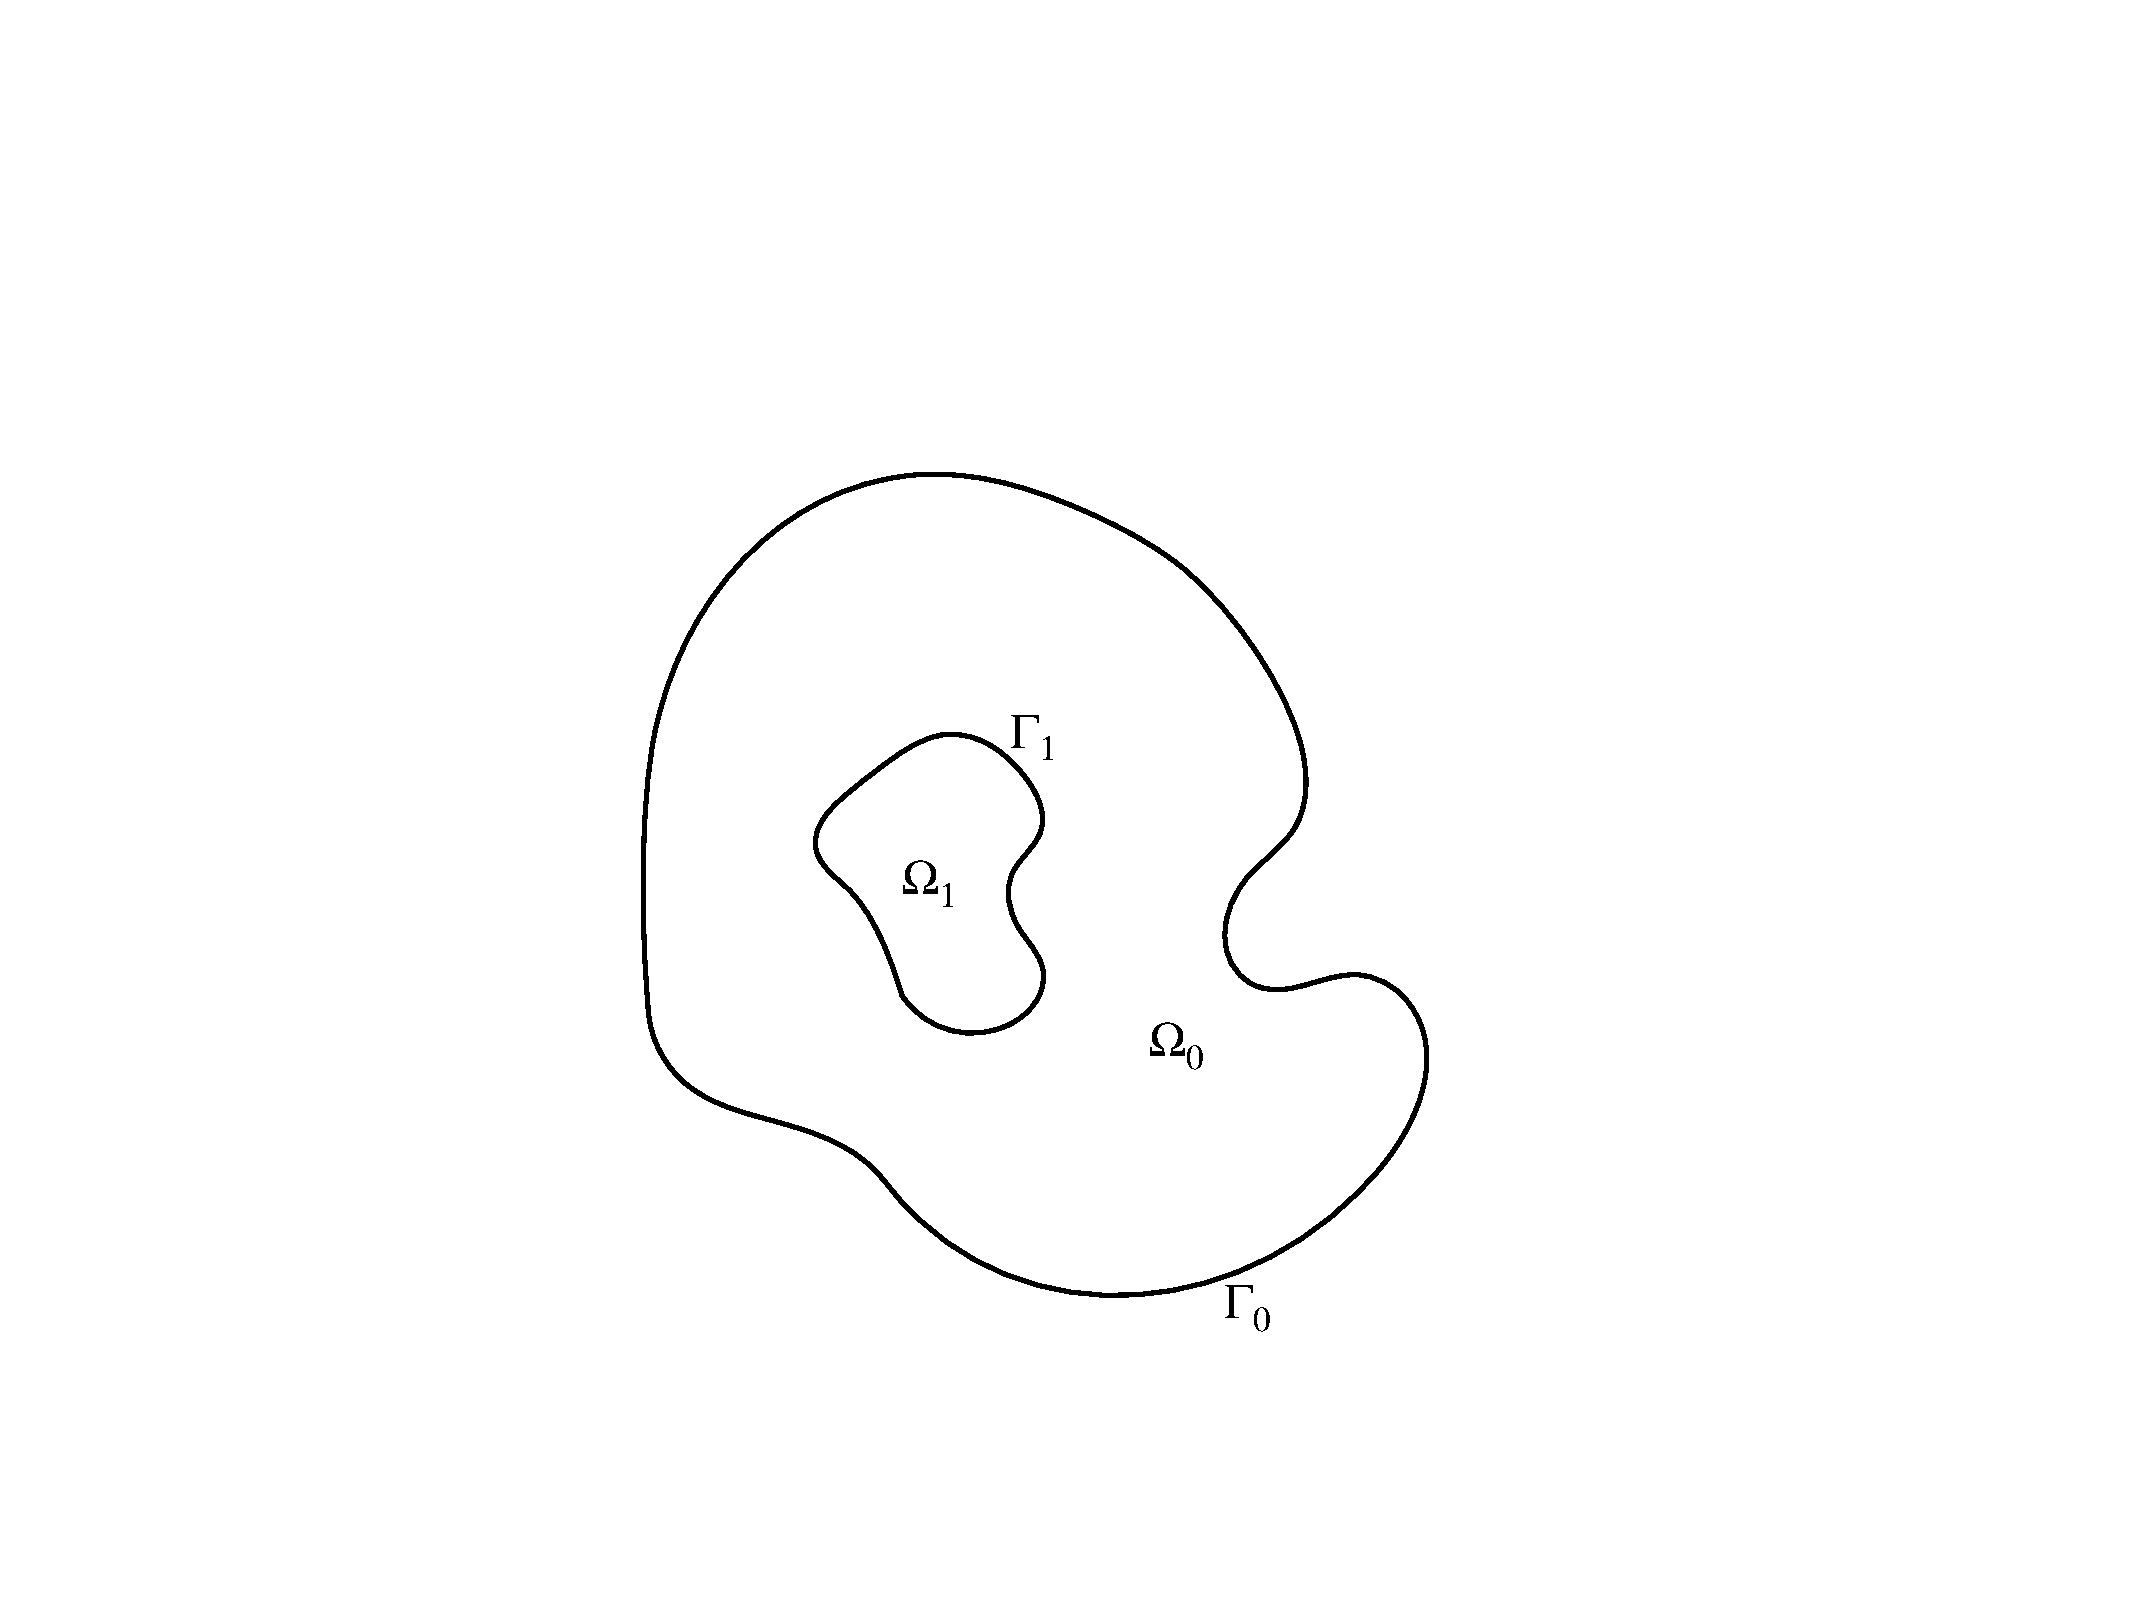
\includegraphics[width=0.3\linewidth]{media/multiply_final}
\end{center}
\caption{Example of a multiply connected domain with one obstacle.}
\label{fig:1ply}
\end{figure}

\begin{proof}
Suppose that $k$ is a Neumann eigenvalue of $\Omega_{1}$. 
$\tilde{\bu}$ be the eigenmode corresponding to this eigenvalue. 
Note that $\tilde{\bu}$ is not identically $0$ on the boundary $\Gamma_{1}$
of $\Omega_{1}$.
Since $\tilde{\bu}$ is an interior Neumann eigenfunction, we note that
the surface traction corresponding to the solution $\bt^{-} = 0$
on the boundary.
Applying Green's identity~\cref{thrm:rep-theorem}, to the solution 
$\tilde{\bu}$ in the interior and taking the interior limit we get
\begin{equation}
\tilde{\bu} = \frac{1}{2}\tilde{\bu} + \cD^{\Gamma_{1}}_{k}[\tilde{\bu}] +
\cS^{\Gamma_{1}} [\bt^{-}] \implies \frac{1}{2} \tilde{\bu} - \cD^{\Gamma_{1}}_{k}[\tilde{\bu}]
= 0\, .
\end{equation}
Note that the sign of the $\bD$ in the representation theorem is switched
since the normal is pointing inwards for the boundary $\Omega_{1}$.
Thus, $\tilde{\bu}$ is a non-trivial null vector of the operator 
$\frac{1}{2}\cI - \cD^{\Gamma_{1}}_{k}$. 
Furthermore since $\tilde{\bu}$ is the boundary data of 
the solution of the oscillatory Stokes equation in $\Omega_{1}$, we
get that $\cW^{\Gamma_{1}}[\tilde{\bu}] = 0$.
Setting $\bmu = \tilde{\bu}$ on $\Gamma_{1}$, and $\bmu = 0$ on $\Gamma_{0}$,
we obtain a non-trivial null vector for the operator $\cI - 2\cD^{\Gamma}_{k} -2\cW^{\Gamma}$
on the boundary $\Gamma = \Gamma_{0} \cup \Gamma_{1}$.
\end{proof}

As noted in~\cite{zhao2015robust}, this lack of one-to-one correspondance between
the invertibility of the integral operator $\cI - 2\cD_{k} - 2\cW$
and the Dirichlet eigenvalues of the Stokes operator on multiply
connected domains causes non-robustness and introduces near 
resonanaces for simply connected domains
which are almost multiply connected.
We demonstrate this issue numerically in~\cref{sec:numanalysis-nearly-mult-con}.

\subsubsection{Mixed layer potential representation}
\label{subsec:mixedanalysis}
The non-robustness of the double layer potential representation
for computing the Dirichlet eigenvalues of Stokes equation can be remdied
by the standard approach of using the mixed layer potential representation,
i.e. setting
$\bu = (\bD_{k} + i\eta \bS_{k})
\bmu$, 
where $\bmu$ is the unknown density to be solved for, and $\eta \in \mathbb{R}^{+}$ 
On imposing the boundary conditions and using~\cref{lem:jump-conds}, 
we obtain the following integral equation on the boundary 
\begin{equation}
(\cI - 2\cD_{k} - 2i\eta \cS_{k}) \bmu = -2 \ff \, . 
\end{equation}
As noted in~\cref{subsubsec:nullspacecorr}, this integral equation 
is also rank-deficient, and we instead use the following 
equivalent integral equation for $\bmu$,
\begin{equation}
(\cI - 2\cD_{k} -2i\eta \cS_{k}  -2\cW)\bmu = -2 \ff \, .
\end{equation}

We now prove that for any bounded region $\Omega$ (simply or multiply
connected) with $C^{2}$ boundaries, there exists a one-to-one correspondance
between the invertibility of the operator
$\cI - 2\cD_{k} - 2i\eta \cS_{k} - 2\cW$ and the Dirichlet eigenvalues
of the Stokes operator on $\Omega$. 

\begin{thrm}
Suppose $\Omega$ is a bounded region defined by the intersection of a 
simply connected domain $\Omega_{0}$ and the exteriors of a finite collection
of bounded simply connected domains $\{ \Omega_{i} \}_{i=1}^{m}$.
As before let $\Gamma_{i}$ denote the boundary of $\Omega_{i}$ and let
$\Gamma = \cup_{i=0}^{m} \Gamma_{i}$ denote the boundary of $\Omega$.
Then the operator $\cI - 2\cD_{k} - 2i\eta \cS_{k} - 2\cW$
is invertible if and only if $k$ is not a Dirichlet eigenvalue
for the Stokes operator on $\Omega$.
\end{thrm}

\begin{proof}
Suppose that $k$ is not a Dirichlet eigenvalue for Stokes equation on
$\Omega$. 
Suppose further that $\bmu$ satisfies
\begin{equation}
(\cI - 2\cD_{k} -2i\eta\cS_{k} - 2\cW) \bmu = 0 \, , \label{eq:mlproofrep}
\end{equation}
i.e. $\bmu$ is in the null-space
of $(\cI - 2 \cD_{k} - 2i\eta \cS_{k} - 2 \cW)$. 
Applying the operator $\cW$ to~\cref{eq:mlproofrep} and 
using~\cref{lem:propnullspacecorr}, we get
\begin{equation}
0 = \cW [(\cI - 2\cD_{k} - 2i\eta\cS_{k} - 2\cW)\bmu] = -2\cW [\bmu] \, .
\end{equation}
Thus~\cref{eq:mlproofrep} reduces to
\begin{equation}
(\cI - 2 \cD_{k} - 2i\eta \cS_{k})\bmu = 0\, .
\end{equation}
Suppose now $\bu = -2\bD_{k}[\bmu] -2i\eta\bS_{k}[\bmu]$ in $\Omega$.
Then $\bu$ is a solution to the oscillatory Stokes equation in $\Omega$,
and applying~\cref{lem:jump-conds}, we get that the interior
limit of the velocity $\bu^{-} = (\cI - 2\cD_{k} -2i\eta\cS_{k}) \bmu = 0$ on $\Gamma$. 
Since $k$ is not a Dirichlet eigenvalue for the Stokes equation on 
$\Omega$, we conclude that $\bu \equiv 0$ in $\Omega$. 
This in particular implies that the interior limit of the surface traction
denoted by $\bt^{-} = 0$ on $\Gamma$.
Using~\cref{lem:jump-conds}  
we observe that the exterior limit 
of the surface traction is $\bt^{+} = i\eta \bmu(\xx)$
and the exterior limit of the velocity is 
$\bu^{+} = \bmu(\xx)$ on $\Gamma$.
\begin{remark}
Note that there is a slight abuse of notation here for the obstacle
boundaries, since the exterior limit with respect to $\Omega$ 
for the boundary $\Gamma_{j}$ is the traditional interior 
limit with respect to the obstacle region $\Omega_{j}$.
\end{remark}
We first show that $\bmu=0$ on $\Gamma_{0}$. 
To this end, note that $\bu$ is a radiating solution of the oscillatory
Stokes equation in the exterior $E$,
since $\cW[\bmu] = 0$ implies that $\int_{\Gamma} \bmu \cdot \bnu = 0$. 
From uniqueness of the impedance problem in the exterior $E$, we conclude
that $\bu \equiv 0$ in $E$ as well, which in particular implies that
the exterior limit of the velocity $\bu^{+}=0$ on $\Gamma_{0}$.   
Using the jump conditions in~\cref{lem:jump-conds} again, we
get that $\bmu = \frac{1}{2}(\bu^{+} - \bu^{-}) = 0$ \, on
$\Gamma_{0}$. 
To show that $\bmu=0$ on $\Gamma_{j}$, we observe that
$\bmu$ is also a solution to the oscillatory Stokes equation
in each of the obstacles $\Omega_{j}$ as well.
Applying Green's identity and using the fact that 
the interior limits with respect to $\Omega_{j}$ (see remark)
of the surface traction and the velocity
are $i\eta \bmu$ and $\bmu$ respectively, we get
\begin{equation}
\int_{\Omega_{j}} (|e(\bu)|^{2} - \overline{k}^{2} |\bu|^2) dV 
= \int_{\Gamma_{j}} \bu \cdot \overline{\bt} dS = 
i\overline{\eta}\int_{\Gamma_{j}} |\bmu|^2 dS \, .
\end{equation}
Taking the imaginary part of the above equation, we get
\begin{equation}
2 \text{Re}(k) \text{Im}(k) \int_{\Omega_{j}} |\bu|^2 + \text{Re}(\eta)
\int_{\Gamma_{j}} |\bmu|^2 dS = 0 \, .
\end{equation}
Since $\text{Re}(\eta)>0$, this implies that $\bmu=0$ for $\xx \in \Gamma_{j}$, $j=1,2,\ldots m$. 
Thus $\cI - 2\cD_{k} -2i\eta\cS_{k} -2\cW$ is invertible when $k$ 
is not a Dirichlet eigenvalue for the Stokes equation on $\Omega$.


From Green's representation for the oscillatory Stokes equation, 
we know that 
  \begin{equation} \label{eq:rep-theorem}
    \bS [\bt](\xx) - \bD[\bu](\xx) = \begin{cases} 
    \bu(\xx) &\quad \xx \in \Omega \, , \\
    0 &\quad \xx \in \Omega^{C} \; .
    \end{cases}
  \end{equation}
Suppose that $k$ is Dirichlet eigenvalue for the Stokes equation on $\Omega$
and let $\bu$ denote the corresponding eigenfunction and let $\bt$ denote
the surface traction associated with the eigenfunction.
Note that the Green's representation theorem implies that 
$\cS_{k}[\bt^{-}] = 0$, since $\bu^{-}=0$ on $\Gamma$. 
Applying the Green's theorem to the pair $\bt^{-}, \bu^{-}$ and taking 
its derivative on $\Gamma$ using~\cref{lem:jump-conds}, we get
\begin{equation}
\bt^{-} = (\cDt_{k} + \frac{1}{2} \cI) \bt^{-} \, . 
\end{equation}
Combining these two identities, we get
that
\begin{equation}
(-\cI - 2\cD_{k} -2i\eta \cS_{k}) \bt^{-} = 0 \, .
\end{equation}
As in the proof of~\cref{thm:dlmain}, letting $c = \left< \bt^{-} ,\bnu \right>$, 
it follows that
\begin{equation}
(-\cI - 2\cD_{k} - 2i \eta \cS_{k} - 2\cW) (\bt^{-} - c\bnu) = 0 \, ,
\end{equation}
where $\bt^{-} - c\bnu \neq 0$.
Since $\bt^{-} - c\bnu$ is non-trivial, and $i\eta \cS_{k}, \cW$ are self-adjoint ($i\eta \cS_{k}$ 
is self-adjoint since we consider inner products without conjugation), 
it follows from the Fredholm alternative 
that the operator $\cI - 2\cD(k) -2i\eta \cS - 2\cW$ is also not invertible.
\end{proof}

\subsection{Fredholm determinants}
Having established the equivalence between the Dirichlet eigenvalues
for Stokes equation and the invertibility of
the operator $\cI - 2\cD_{k} - 2\cW$ on simply connected domains, in this section
we show how the Fredholm determinant can be as a computational tool for detecting
the non-invertibility of $\cI - 2\cD_{k} - 2\cW$.

Let $\cJ_{1}(X)$ denote the space of trace class operators 
on $X$, where $X$ is a Hilbert space.
$\cJ_{1}$ is a subspace of compact operators on $X$.
Suppose that $A$ is a compact operator, with eigenvalues
$\lambda_{i}, i\in \mathbb{N}$.
Then the operator $A \in \cJ_{1}(X)$ if
$\sum_{i} |\lambda_{i}| < \infty$.
If $A$, is a trace class operator, then  
the Fredholm determinant of the operator $\cI + A$ is defined as
\begin{equation}
\text{det}(\cI +A) = \prod_{i=1}^{\infty} (1+\lambda_{i}) \, .
\end{equation}
It follows from standard results in complex analysis, 
that the Fredholm determinant is finite and well-defined if 
$\text{det}(\cI+A) < \infty$ if $\sum_{i} |\lambda_{i}| < \infty$,
i.e. if $A$ is in trace class.

The following lemma shows that the operator 
$-2\cD_{k} - 2\cW$ is a trace class operator.
\begin{lemma} 
$-2\cD_{k} - 2\cW$ is a trace class operator for all $k$ 
\end{lemma}
\begin{proof}
Using Bessel function asymptotics, we note that the
kernel of $\cD_{k}$ given by
$\TT_{\cdot,\cdot,\ell}\nu_{\ell}(\bx,\by)$
has a leading order singularity of $|\bx-\by|^2 \log{|\bx-\by|^2}$ as $\bx\to \by$.
It follows from~\cite{bornemann2010numerical} numerical that $\cD_{k}$
is a trace-class operator for all $k$.
Since $\cW$ is a rank-one perturbation independent of $k$, and trace-class
operators are a vector space, we conclude that
$-2\cD_{k} - 2\cW$ is also a trace-class operator for all $k$.
\end{proof}

Let $f(k) = \text{det}(\cI - 2\cD_{k} - 2\cW)$.
We first note that $f(k)$ is an analytic function of $k$
for $k \in \mathbb{C} \setminus 0$
since the kernel of $\cD_{k}$ is an 
analytic function of $k$ on that domain, 
and the Fredholm determinant is an analytic operator.

The Fredholm determinant of a second-kind Fredholm operator
is another way of detecting when the operator is not invertible. 
The following result summarizes the result. 
\begin{lemma}
$f(k) = 0$ if and only if $\cI - 2\cD_{k} -2\cW$ 
is not invertible.
\end{lemma}
\begin{proof}
The proof is standard and see for example~\cite{simon2005trace}, page 34.
\end{proof}

When $\Omega$ is simply connected, the above lemma combined 
with~\cref{thm:dlmain} implies $f(k) = 0$ if and only if $k$ 
is a Dirichlet eigenvalue for Stokes equation.

We now show how this fact can be used numerically
to estimate the Dirichlet eigenvalues.
Suppose that $M_{k}^{N}$ is a Nystr\"{o}m discretization 
of the operator $-2\cD_{k} - 2\cW$ when the boundary 
$\Gamma$ is discretized with $N$ points. 
Let $f^{N}(k) = \text{det}(I + M_{k}^{N})$
where here $\text{det}$ is the standard matrix determinant.
Note that the discretized matrix also depends on the choice
of quadrature rule used in the Nystr\"{o}m discretization
of the operator.


In~\cite{zhao2015robust}, the authors prove that
for computing the Laplace eigenvalues on regions with 
analytic boundaries, when the integral
operators are discretized using Kress-quadrature~\cite{kress1991boundary},
the determinant of the Nystr\"{o}m discretized operators
at the true eigenvalues converge to $0$ exponentially in $N$.
Thus, if the eigenvalues have multiplicity $1$, i.e. the
derivative of the determinant is non-zero at the true-eigenvalues,
then the analyticity of the discretized determinant implies
that the zeros of the determinant of the Nystr\"{o}m 
discretization of the linear operator converge
exponentially to the true Dirichlet eigenvalues for Laplace's equation.

The proof presented in~\cite{zhao2015robust} carries forward
for computing the Dirichlet eigenvalues of Stokes equation as well.
We summarize the result in the following theorem.
\begin{thrm}
\label{thm:mainconvfreddet}
Suppose that $\Omega$ is a simply connected domain with an analytic boundary.
Let $k_{j}$, $j=1,2,\ldots M$ denote all the Dirichlet eigenvalues of Stokes
equation on $\Omega$ contained in the interval $[a,b]$. 
Suppose further that all the eigenvalues have multiplicity $1$.
Let $f^{N}(k) = \text{det}(I+M^{N}_{k})$, where $M^{N}_{k}$ 
is the Nystr\"{o}m discretzation of $-2\cD_{k} - 2\cW$ with Kress
quadrature.
Then $f^{N}(k)$ has exactly $M$ zeros on the interval $[a,b]$. 
Let $\omega_{j}$, $j=1,2\ldots M$ denote the zeros of $f^{N}$.
Furthermore, there exist constants $a>0$ and $C$, 
such that $\sup_{j=1}^{M} |\omega_{j} - k_{j}| < C e^{-aN}$.
\end{thrm}

\begin{proof}
The proof follows from small modificiations of the proofs contained in~\cite{zhao2015robust}. 
\end{proof}

In practice, using Kress-quadrature for large problems is problematic owing to the global
nature of the quadrature rule. 
The coupling with fast direct solvers for computing determinants also results in $O(N^2 \log{N})$ 
determinant evaluation since evaluating each matrix entry costs $O(N)$, where 
$N$ is the number of discretization points on the boundary.
Over the last two decades, many high-order quadrature methods which are compatible with
fast algorithms like the fast multipole method (and fast direct solvers as well, 
since each matrix entry requires O(1) work) have been developed for solving
integral equations.
Extensive numerical evidence suggests that the zeros of the 
determinants of linear systems discretized using 
these quadrature methods are also high order approximations of Dirichlet eigenvalues
for the Stokes PDE--- the error is observed to be proportional to the quadrature error
for the eigenfunction $\bt^{-}$ associated with the eigenvalue.
We leave a proof of this to future work.


\begin{remark}
The same analysis does not carry through for the operator
$\cI - 2 \cD_{k} - 2i\eta \cS_{k} - 2\cW$, 
since $\cS_{k}$ is not a trace class operator.
For brevity, let $\cM_{k} = -2\cD_{k} - 2i\eta \cS_{k} - 2\cW$.
The operator $\cM_{k}$ is 
in $\cJ_{2}(\bL^{2}(\Gamma))$ where
$\cJ_{2}(\bL^{2}(\Gamma))$ is the space of Hilbert-Schmidt operators
on $\bL^{2}(\Gamma)$ (the singular values of the operator are square
summable, as opposed to being summable).
Thus the Fredholm determinant of $\cI + \cM_{k}$
is not necessarily finite. 
However, as noted in~\cite{zhao2015robust}, the convergence
result~\cref{thm:mainconvfreddet}
should be true up to a logarithmic factor in the rate
of convergence, since the singular values of the operator
$\cM_{k}$ decay like $\frac{1}{n}$, and the
Fredholm determinant divergers logarithmically. 
In~\cref{subsec:convannulus}, we demonstrate that this fact
numerically on the annulus, where the eigenvalues are analytically known. 
\end{remark}

\section{Numerical Results}
\label{sec:numerical}

In this section, we demonstrate the analytical
claims above with numerical examples and
highlight the performance of the BIE approach
to Stokes eigenvalues.

\subsection{Numerical methods}

First, we describe the numerical tools needed
to compute Stokes eigenvalues in a BIE
framework.

\subsubsection{Discretizing the BIE}

In order to turn the BIEs analyzed
above into discrete linear systems,
we require some standard techniques
from the BIE literature.

Let the boundary be divided into $N_p$
panels.
%
We parameterize panel $j$ as
$\bx_j(t)$, with $t$ ranging over the
interval $[-1,1]$.
%
Each component of $\bx_j$ is taken to be
a polynomial interpolant over the
standard 16th-order Legendre nodes on
$[-1,1]$, denoted by $t_n$, so that
the total number of discretization
points is $N=16N_p$.
%
See \cref{fig:panels} for an example
discretization.
%
Another important quantity below is the
arc-length density of a panel, which
we denote by $s_j(t) := |\bx'_j(t)|$.
%
Finally, we denote the set of panels
which are adjacent to panel $j$
by $A(j)$. On a closed curve,
$A(j)$ contains two integers.

The integral kernels of the single and
double layer potentials have weak
singularities of the form $r^p\log r$
which require special quadrature rules to
achieve high-order accuracy.
%
In the examples below, we use generalized
Gaussian quadrature (GGQ)~\cite{bremer2010}.
%
To demonstrate the idea, we consider
evaluating the convolution of a kernel
$K$ with a density $\sigma$
at the boundary node $\xx_j(t_l)$.
%
GGQ is a Nystr\"{o}m-type discretization ---
the density is approximated 
by its values at the discretization nodes,
which we denote by
$\sigma_{qp} := \sigma(\xx_q(t_p))$.
%
The basis of a GGQ rule is a set of 
support nodes and weights for the
contribution to the integral from the
``self'' panel (panel $j$) and the adjacent
panels (with index in $A(j)$).
%

For the self panel, there is a special set
of nodes and weights for each interpolation
point. Denote the nodes and weights
for interpolation point $l$ by $t^{(l)}_{n}$
and $w^{(l)}_{n}$, respectively, with
$1\leq l \leq 16$ and $1\leq n \leq N_s$.
%
The adjacent panels are handled by a single
set of over-sampled support nodes and weights.
We denote these nodes and weights
by $\tilde{t}_n$ and $\tilde{w}_n$, respectively,
for $1 \leq n \leq N_a$.
%
For the rules we used, $N_s = 16$ and
$N_a = 48$.
%
The contribution of other panels is assumed
to be given to high accuracy by the standard
Gauss-Legendre weights, which we denote
by $w_n$.
%
Adding these contributions together, we obtain the
quadrature

\begin{multline}
  \int_\Gamma K(\xx_i(t_l),\yy) \, \sigma(\yy)
  \, dS(\yy) \approx \\
  \sum_{p=1}^{16} \sum_{n=1}^{N_s}
  w^{(l)}_{n} K(\xx_i(t_l),\xx_i({t}^{(l)}_{n}))
  s_i({t}^{(l)}_{n}) B^{(l)}_{np} \sigma_{ip} \quad \textrm{(self)}
  \\
  + \sum_{q\in A(i)} \sum_{p=1}^{16} \sum_{n=1}^{N_a}
  \tilde{w}_jK(\xx_i(t_l),\xx_q(\tilde{t}_n)) s_q(\tilde{t}_n)
  C_{np} \sigma_{qp}
  \quad \textrm{(adjacent)} \\
  + \sum_{q\neq i, q\not\in A(i)} \sum_{p=1}^{16}
  w_p K(\xx_i(t_l),\xx_q(t_p)) s_q(t_p)
  \sigma_{qp} \quad \textrm{(far)} \nonumber \; ,
\end{multline}
where $\bB^{(l)}$ and $\bC$ are interpolation
matrices from the standard Legendre nodes
to the self and adjacent panel support nodes,
respectively. Observe that the quadrature is
linear in $\sigma_{qp}$. In practice, we pre-compute
and store the self and adjacent matrix entries for each
interpolation point, which is a parallelizable
$O(N)$ calculation. The ``far'' interactions
are computed on-the-fly.

\begin{remark}
  \label{rmk:levelrestrict}
  We ensure that ``far'' interactions
  are handled to high precision by requiring that
  no two adjacent panels differ in length
  by more than a factor of 2. On a domain which does
  not nearly self-intersect this
  guarantees that no ``far'' interactions occur
  which are much closer than 1/2 of a panel away
  (assuming panels are relatively flat).
  Because the location of the singularity is
  bounded away from the panel and the smooth
  rule is of high order, we obtain a quadrature
  rule with sufficient precision.
\end{remark}

\subsubsection{Fast determinant method}

Once the discretization is set, we can form
a compressed representation of the system matrix
using recursive skeletonization~\cite{ho2012fast}.
%
We use the implementation of this procedure
included in the fast linear algebra in
MATLAB (\texttt{FLAM}) package
\cite{hoFLAM_1253582}.
%
At low-to-medium frequencies, the scaling
of the recursive skeletonization algorithm
is $O(N\log N)$ in operation count and
storage and, by using a generalization
of the Sylvester determinant formula,
allows for a fast determinant
calculation in $O(N\log N)$ time as a
follow-up step.
%
At higher-frequencies,
the recursive skeletonization procedure,
which is based on the assumption that off-diagonal
blocks of the matrix are of low rank,
breaks down and does not offer a speed advantage.
%
These algorithms take a precision parameter
$\epsflam$ which determines the
accuracy to which any sub-blocks of the matrix
should be compressed. In all experiments,
we set $\epsflam = 10^{-14}$.

The compressed representation also allows
for fast applications of the system matrix,
its transpose, the inverse of the system
matrix, and the inverse transpose to
vectors.
%
In particular, this allows us to estimate the
smallest singular values by performing
randomized subspace iteration, see
\cite[Algorithm 4.4]{halko2011finding},
on the inverse operator.
%
Below, we use the smallest singular value
as a measure of the quality of the
eigenvalues found by approximating the
roots of the determinant.
%
We also evaluate the second smallest singular
value if the root finding precedure suggests a
possible double root. 

\subsubsection{Interpolation and root-finding}

To estimate the eigenvalues, we fit a Chebyshev
interpolant to the discretized determinant as a
function of $k$ on intervals.
%
This is done adaptively so that the Chebyshev
coefficients of the determinant have decayed
to the point that the ratio of the last
coefficient to the largest coefficient is below
some threshold.
%
In all experiments, we set this threshold
as $\epscheb = 10^{-13}$.
%
We perform this fit using the \texttt{chebfun}
utility in the package of the same name
\cite{driscoll2014chebfun}
so that we can make use
of the \texttt{roots} utility to approximate
the roots of the determinant.

The \texttt{roots} utility returns the roots
of the polynomial in the complex plane, with
some minimal internal processing to remove
spurious roots.
%
Because our numerical determinant evaluation
is somewhat noisy and we fit the function up to
precision $\epscheb$, we perform some
further post-processing to eliminate remaining
spurious roots.
%
Let $k^{(l)}_\cheb$ denote the roots of the interpolants.
%
We ignore any of the returned roots with $|\imag(k^{(l)}_\cheb)|
> \sqrt{\epscheb}$, as these are too far from real-valued
to be non-spurious.
%
For the remaining roots, we consider the
properties of $\real(k^{(l)}_\cheb)$.
%
We inspect any pairs of roots $(k^{(p)}_\cheb,k^{(q)}_\cheb)$
for which $|\real(k^{(p)}_\cheb-k^{(q)}_\cheb)| < \sqrt{\epscheb}$,
as these are possibly spurious double roots.
%
For these pairs, we compare the right singular
vector of the appropriate BIE operator corresponding
to the smallest singular value for each of $\real(k^{(p)}_\cheb)$
and $\real(k^{(q)}_\cheb)$, which we denote by
$\bv_p$ and $\bv_q$.
%
If $\|\bv_p - \bv_q \bv_q^* \bv_p \| < 10^{-5}$, then
we consider the pair to be spurious.
%
For these near double roots, we also check
that there is no two dimensional null-space
corresponding to the root by estimating the
second smallest singular value of the BIE operator.
%
If this is larger than $10^{-5}$, then we declare
it to be a simple root.

We can obtain an a posteriori estimate of the
error in a computed root as follows.
%
Let $f$ denote an analytic function,
$P$ be the polynomial interpolant
of that function over some interval,
$\delta f = f-P$ be the difference,
and $k_\cheb$ denote a computed root
of $P$ which is simple (i.e. assume
that $P'(k_\cheb) \ne 0$).
%
The algorithm used by \texttt{chebfun}
to approximate the roots of $P$ is
backward stable~\cite{noferini2017chebyshev}.
Therefore the error in the roots will be
small relative to the error of the fit and
we set $P(k_\cheb) = 0$ below.
%
Suppose that
$f(k_\cheb + \delta k) = 0$ for some
small $\delta k$. Then

\begin{align*}
  0 &= f(k_\cheb + \delta k) \\
  0 &= P(k_\cheb + \delta k) + \delta f(k_\cheb + \delta k) \\
  \delta k &= -\frac{\delta f(k_\cheb + \delta k)}{P'(k_\cheb)} + O(\delta k^2) .
\end{align*}
In practice, we can obtain an approximate upper
bound for $|\delta f(k_\cheb+\delta k)|$
as $\epscheb \|P\|_\infty$ so that $\epscheb \|P\|_\infty/
|P'(k_\cheb)|$ provides an approximate upper bound
for the error in the root.

\subsection{Eigenvalues of an annulus}
We test our numerical machinery and validate our analytical 
and numerical claims
by comparing the results to the true eigenvalues on the annulus
which are known analytically (see~\cref{sec:annul_dir_exact}).
In all of the examples below, we work on the annulus $r_{1}<r<r_{2}$
with $r_{1} = 1$ and $r_{2} = 1.7$.
If the inner boundary is discretized using $N_{1}$ panels, 
then the outer boundary is discretized using $N_{2} = 
\lceil r_{2}/r_{1} N_{1} \rceil +1$ panels to ensure that the
panels are approximately the same length on both the boundaries. 
The total number of discretization points 
is then given by $N = 16(N_{1} + N_{2})$.
Let $D^{N}_{k}$ denote the linear system corresponding
to the Nystr\"{o}m discretization of
$-2\cD_{k} -2\cW$ using generalized Gaussian quadrature, 
and let $C^{N}_{k}$ denote the linear system corresponding
to the Nystr\"{o}m discretization of 
$-2\cD_{k} - 2i\cS_{k} -2\cW$.
Let $f_{D}^{N}(k) = \text{det}(I+D^{N}_{k})$, and 
$f_{C}^{N}(k) = \text{det}(I+C^{N}_{k})$.

\subsubsection{Convergence study}
\label{subsec:convannulus}
We demonstrate that 
for sufficiently large $N$, if $k_{0}$ is a Dirichlet 
eigenvalue of the annulus, 
then $f_{D}^{N}(k_{D}) = 0$ and $f_{C}^{N}(k_{C}) = 0$
where $|k_{D} - k_{0}| \lsim N^{-20}$, 
and $|k_{C} - k_{0}| \lsim N^{-20}$.
Note that N^{-20} is the observed order of
convergence for Generalized Gaussiuan quadratures for weakly 
singular integrals.
In~\cref{fig:conv}, we show this result for $k_{0} = 13.48025717955055$
and plot the errors $|k_{D}-k_{0}|$ and $|k_{C}-k_{0}|$ as a function
of $N$. 

\subsubsection{Spurious eigenvalues}
\label{subsec:spurannulus}
As noted in~\cref{subsec:dlanalysis},
if $k_{0}$ is a Neumann eigenvalue corresponding to the interior
inclusion, which in our case is the disk $r\leq r_{1}$, then
$f_{D}(N)(k_{0}) is O(\varepsilon)$ even though $k_{0}$ 
is not a Dirichlet eigenvalue of the annulus, i.e.
the integral equation $-\cI - 2\cD_{k} -2\cW$ has a spurious eigenvalue.
In~\cref{fig:spur}, we demonstrate this result and also show that 
$f_{C}^{N}(k_{0}) \neq 0$, i.e., the combined field representation is
robust and invertible at all values of $k$ which are not the Dirichlet
eigenvalues of the annulus. 

\subsubsection{Speed}
\label{subsec:speed}
In this section, we demonstrate the O(N\log{N}) scaling of evaluating
$f^{N}_{C}(k)$ as long as $N$ is large enough to resolve the interactions
at the Helmholtz parameter $k$. 
When $N$ is smaller than that, we observe a worse scaling since the
assumption that far-interactions are low-rank is no longer valid at
the tolerance of FLAM.
We plot the timing results corresponding to three different values of 
$k$ in~\cref{fig:speed}.


\subsection{Eigenvalues of a barbell-shaped domain}
\label{subsec:barbell}

\begin{figure}
  \centering
  \begin{subfigure}[t]{0.4\textwidth}
    \centering
    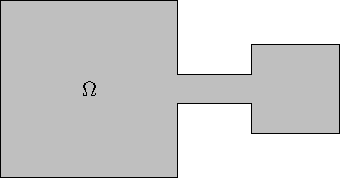
\includegraphics[width=\textwidth]{fig/ex_barbell_001_bdry}
    \caption{A barbell-shaped domain.}
    \label{subfig:barbell_bdry}
  \end{subfigure}
  ~
  \begin{subfigure}[t]{0.4\textwidth}
    \centering
    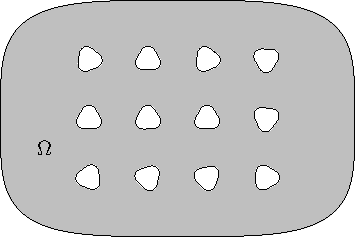
\includegraphics[width=\textwidth]{fig/ex_many_holes_004_bdry}
    \caption{A domain with several inclusions.}
    \label{subfig:many_inclusions_bdry}
  \end{subfigure}
\end{figure}

\begin{figure}
  \centering
  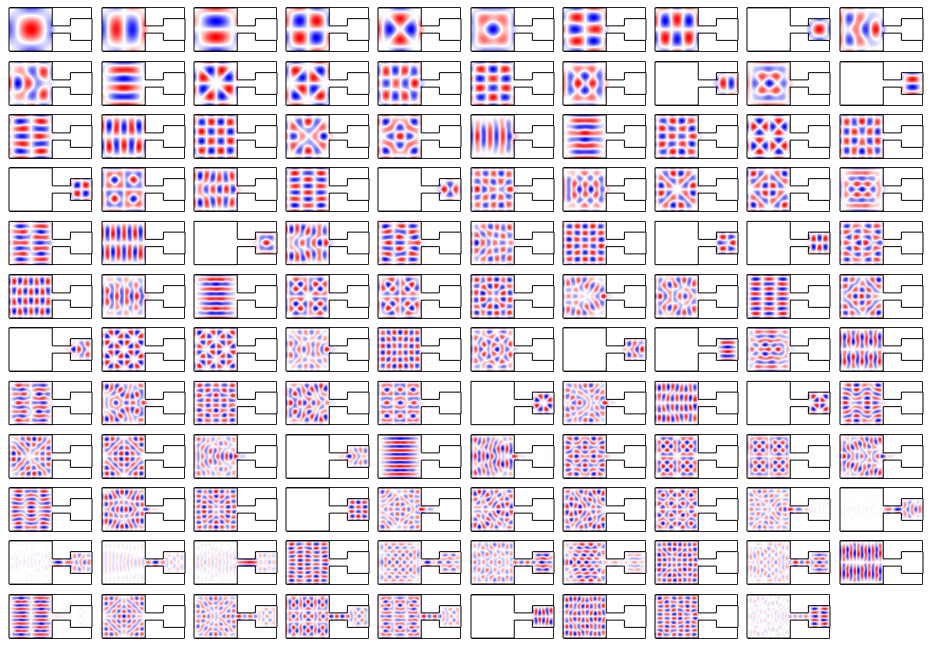
\includegraphics[width=\textwidth]{fig/barbell_gallery}
  \caption{Vorticity plots of the first 119 eigenfunctions
    of the barbell-shaped domain.}
  \label{fig:barbell_gallery}
\end{figure}

\begin{figure}
  \centering
  \begin{subfigure}[t]{0.4\textwidth}
    \centering
    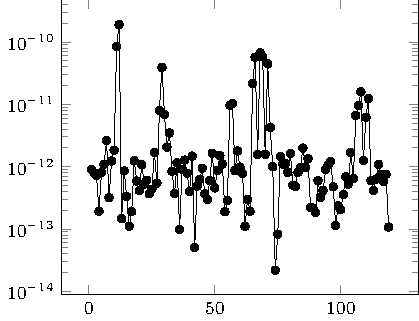
\includegraphics[width=\textwidth]{fig/ex_barbell_001_sings_plot}
    \caption{Smallest singular value of the BIE operator.}
    \label{subfig:barbell_sings}
  \end{subfigure}
  ~
  \begin{subfigure}[t]{0.4\textwidth}
    \centering
    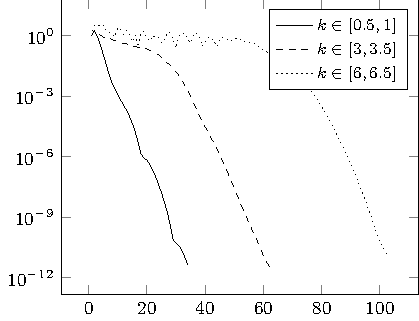
\includegraphics[width=\textwidth]{fig/ex_barbell_001_coeffs_plot}
    \caption{Normalized Chebyshev coefficients of the
      determinant on 3 intervals in $k$.}
    \label{subfig:barbell_coeffs}
  \end{subfigure}
  \caption{Diagnostics for the first 119 barbell eigenvalues.}
  \label{fig:barbell_diagnostics}
\end{figure}

We consider the barbell-shaped domain in \cref{subfig:barbell_bdry}.
This domain is the union of a square of side-length 6,
a square of side-length 3, and a ``bridge'' connecting
them of height 1 and width 5/2.
%
For the sake of simplicity, we round the corners of the domain
to obtain a smooth object.
%
Applying the approach described in~\cite{epstein2016smoothed},
the corners of the domain are rounded by convolving with
the Gaussian kernel
\begin{equation}
  \nonumber
\phi(x) = \frac{1}{\sqrt{2\pi h}} e^{-x^2/(2 h^2)} \, ,
\end{equation}
with $h\approx 0.06$. This leaves the domain unperturbed
to high precision outside of a radius of $0.1$ around
each corner.
%
The eigenfunctions of such a domain display the well-known
localization property~\cite{trefethen2006computed}:
many of the eigenfunctions are approximately supported
within one of the squares.
%
We compute these eigenfunctions corresponding to
eigenvalues $k^2$ with $k$ in the range
$0.5 \leq k \leq 6.5$.

%
The panels are divided adaptively so that the smallest
panels in the rounded corners are smaller than $10^{-2}$,
which keeps the panels relatively flat.
%
This results in $N_p = 412$ after enforcing the
level-restriction property described in
\cref{rmk:levelrestrict}
and enforcing that no panel is larger than
one wavelength for the largest $k$
(here $\lambda=2\pi/6.5$).

As this is a simply-connected domain,
the eigenvalues are estimated by finding the values
$k$ for which $\cI-2\cDk-2\cW$ is non-invertible.
%
Let $f^N(k) = \det (\cI^N-2\cDk^N-2\cW^N)$.
To find the roots of $f^N(k)$, we fit a \texttt{chebfun}
representation of $f^N(k)$ on each of the intervals
$[j/2,(j+1)/2]$ for $j = 1,\ldots,12$.
%
We plot the absolute value of the Chebyshev coefficients
(normalized by the absolute value of the first coefficient)
of $f^N(k)$ on the intervals $[0.5,1.0]$, $[3.0,3.5]$,
and $[6.0,6.5]$ in \cref{subfig:barbell_coeffs}.
%
As expected, the coefficients decay exponentially
to zero, with more terms required at higher
frequencies.
%

We compute the roots of these Chebyshev interpolants
and apply the post-processing described above.
%
There were 135 total roots: 3 were removed because
the imaginary part was too large and 13 pairs were found
with values within $\sqrt{\epscheb}$ of each other.
%
For these 13 pairs, none represented two distinct
eigenvalues or a double root.
%
This leaves 119 roots in the range $0\leq k \leq 6.5$.
%
We plot the smallest singular value of
$\cI^N-\cDk^N-2\cW^N$ for each of these roots in
\cref{subfig:barbell_sings}
and plot the vorticity of the eigenfunctions
in \cref{fig:barbell_gallery}.
%
The singular values suggest that the quality of the
eigenvalues is good.
From the plots, we see that localization occurs
until about the 100th eigenvalue.

%

%\subsection{Robustness on a nearly multiply connected domain}
%\label{subsec:crescent}

\subsection{Eigenvalues of a domain with several inclusions}

\begin{figure}
  \centering
  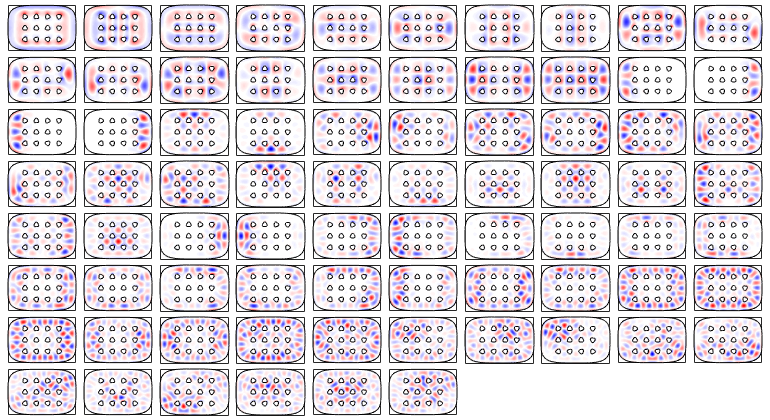
\includegraphics[width=\textwidth]{fig/many_inclusions_gallery}
  \caption{Vorticity plots of the eigenfunctions corresponding
  to the first 76 eigenvalues of a domain with several inclusions.}
  \label{fig:many_inclusions_gallery}
\end{figure}

\begin{figure}
  \centering
  \begin{subfigure}[t]{0.4\textwidth}
    \centering
    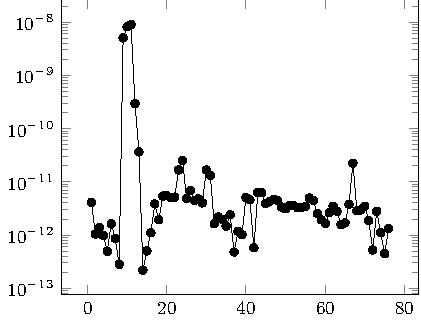
\includegraphics[width=\textwidth]{fig/ex_many_holes_004_sings_plot}
    \caption{Smallest singular value of the BIE operator
      corresponding to the first 76 eigenvalues of a
      domain with several inclusions.}
    \label{subfig:many_inclusions_sings}
  \end{subfigure}
  ~
  \begin{subfigure}[t]{0.4\textwidth}
    \centering
    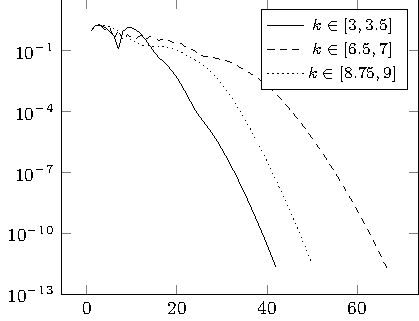
\includegraphics[width=\textwidth]{fig/ex_many_holes_004_coeffs_plot}
    \caption{Normalized Chebyshev coefficients of $f^N(k)$ on
      3 different intervals in $k$.}
    \label{subfig:many_inclusions_coeffs}
  \end{subfigure}
  \caption{Diagnostics for the eigenvalues of a domain
    with several inclusions.}
  \label{fig:many_inclusions_diagnostics}
\end{figure}

We now consider the multiply-connected domain in
\cref{subfig:many_inclusions_bdry}.
% 
The domain is defined by a smooth rectangular region
of width 3 and height 2,
with an array of randomly rotated ``starfish'' shapes
removed. 
%
Such shapes are of interest in
materials design and micro-fluidics \note{cite}.
%
We compute the eigenfunctions corresponding to
eigenvalues $k^2$ with $k$ in the range
$3 \leq k \leq 9$ (this range includes the smallest
eigenvalue).

%
For this smooth shape, ensuring that no panel is
larger than one wavelength for the largest $k$
(here $\lambda=2\pi/9$) is sufficient to resolve
the object to high precision.
%
After enforcing the
level-restriction property described in
\cref{rmk:levelrestrict}, we end up with
$N_p = 224$.

As this is a multiply-connected domain,
the eigenvalues are estimated by finding the values
$k$ for which $\cI-2\cDk-2i\cSk-2\cW$ is non-invertible.
%
Let $f^N(k) = \det (\cI^N-2\cDk^N-2i\cSk^N-2\cW^N)$.
To find the roots of $f^N(k)$, we fit a \texttt{chebfun}
representation of $f^N(k)$ on each of the intervals
$[j/2,(j+1)/2]$ for $j = 6,\ldots,13$ and the intervals
$[j/4,(j+1)/4]$ for $j = 28,\ldots,35$.
%
It should be noted that, due to the relative sizes
of the domains,
this represents a lower frequency problem than
that for the barbell when measured in the number
of wavelengths across the object.
%
Thus, the use of a finer grid in frequency results from
the difficulty in resolving the Fredholm determinant
for this problem, which has a larger dynamical range
than that for the barbell.
%
We plot the absolute value of the Chebyshev coefficients
of $f^N(k)$ on the intervals $[3,3.5]$, $[6.5,7]$,
and $[8.75,9]$ in \cref{subfig:barbell_coeffs}.
%
As expected, the coefficients decay exponentially
to zero, with more terms required at higher
frequencies (note that the interval $[8.75,9]$ is
smaller than the others).
%

We compute the roots of these Chebyshev interpolants
and apply the post-processing described above.
%
There were 103 total roots: 21 were removed because
the imaginary part was too large and 6 pairs were found
with values within $\sqrt{\epscheb}$ of each other.
%
For these 6 pairs, none represented two distinct
eigenvalues or a double root.
%
This leaves 76 roots in the range $0\leq k \leq 9$.
%
We plot the smallest singular value of
$\cI^N-\cDk^N-2i\cSk^N-2\cW^N$ for each of these roots in
\cref{subfig:many_inclusions_sings}
and plot the vorticity of the eigenfunctions
in \cref{fig:many_inclusions_gallery}.
%
In the vorticity plots, we observe a different type of
localization property than that seen in the barbell,
with many of the eigenfunctions
approximately supported in a small, connected subset
of the domain. This is consistent with other studies
\note{cite}

%

\begin{figure}
  \centering
  \begin{subfigure}[t]{0.4\textwidth}
    \centering
    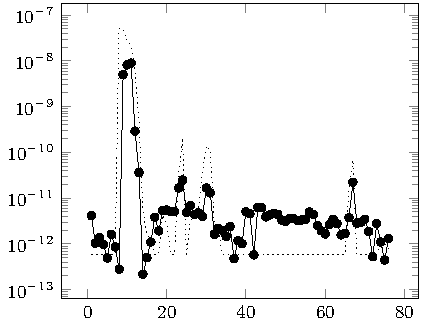
\includegraphics[width=\textwidth]{fig/ex_many_holes_004_sings_plot_west}
    \caption{Smallest singular value of the BIE operator
      for the computed roots (original intervals)
      along with an estimate of the error in the root (dotted).}
    \label{subfig:many_inclusions_sings_west}
  \end{subfigure}
  ~
  \begin{subfigure}[t]{0.4\textwidth}
    \centering
    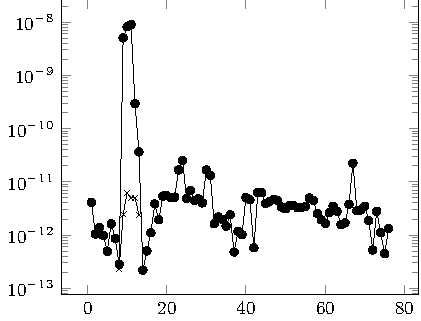
\includegraphics[width=\textwidth]{fig/ex_many_holes_004_sings_plot_ref}
    \caption{Smallest singular value of the BIE operator
      for the computed roots on the original intervals (\textbullet)
      and the values obtained on the refined interval ($\times$).}
    \label{subfig:many_inclusions_sings_ref}
  \end{subfigure}
  \caption{Further diagnostics for the eigenvalues of a domain
    with several inclusions.}
  \label{fig:many_inclusions_diagnostics_2}
\end{figure}

The singular values suggest that the quality of the
eigenvalues is good, with a few outliers.
%
To explain these outliers, we consider two quantities
which affect the singular value at a computed root.
%
As described above, we can approximate the
error in the computed root at $k_\cheb$ by
$\epscheb \|P\|_\infty/|P'(k_\cheb)|$,
where $P$ is the interpolating polynomial.
%
The singular value estimate itself is affected by
the error incurred in applying the inverse of the
compressed BIE matrix, which can be hard to quantify
\cite{ho2012fast}.
%
We approximate this error by $O(\sqrt{N})\epsflam$
and assume this is the order of the error in
the singular value estimate.
We plot the maximum of these two estimates
along with the computed singular values in
\cref{subfig:many_inclusions_sings_west}.
There is a reasonably good correlation between
the maximum of the error estimates and the
observed smallest singular value for the BIE,
especially for larger errors.

The worst outliers are from the left half
of the interval $[4.5,5]$.
%
Because the determinant is much larger on the
right half than the left half of $[4.5,5]$,
we can improve the estimate for the error
in the roots by subdividing the interval. 
We plot the smallest singular value of the
BIE for the roots obtained by fitting a polynomial
on $[4.5,4.75]$ in \cref{subfig:many_inclusions_sings_ref};
the roots on the refined interval
are of significantly higher quality.

\begin{remark}
  The above experience suggests that
  the ratio $\|P\|_\infty/|P'(k_\cheb)|$
  is a useful diagnostic for performing
  automated eigenvalue estimation.
  Note that at a multiple root, this ratio
  will be more difficult to bound.
\end{remark}
%



%

\bibliographystyle{plain}
\bibliography{refs}

\end{document}
